%%****************************************************************************
%** Copyright 2002, 2003 by Lukas Ruf, <ruf@topsy.net>
%** Information is provided under the terms of the
%** GNU Free Documentation License <http://www.gnu.org/copyleft/fdl.html>
%** Fairness: Cite the source of information, visit <http://www.topsy.net>
%****************************************************************************
%** Last Modification: 2013-07-31
%** 2005-07-11	Bernhard Tellenbach
%**							Switched default document class to: book
%**							Added %%****************************************************************************
%** Copyright 2005 by Bernhard Tellenbach, <bernhard.tellenbach@airmail.ch>
%** Information is provided under the terms of the
%** GNU Free Documentation License <http://www.gnu.org/copyleft/fdl.html>
%****************************************************************************
%****************************************************************************
%** Last Modification: 2005-07-11 1600
%** 2005-07-11	Updated the syntax to match the current nomencl packet
%****************************************************************************

\chapter{\label{appendixMessagingProtocol}Relay Messaging Protocol}
The following table shows the exact specification of the different message types used in the \textit{relay protocol}. The field sizes and the communication directions are given in the corresponding columns.

\begin{center}
\begin{tabular}{|l|l|l|l|}
	\hline
	\textbf{Message Type} & \textbf{Communication} & \textbf{Size (bits)} & \textbf{Field} \\
	\hline
	REY	& C $\leftrightarrow$ S 	& 24		& Command (=REY) \\
		& 		& 4		& Flag \\
		& 		& 20		& Secret \\
	\hline
	INV	& M $\to$ C 	& 24		& Command (=INV) \\
		& 		& 256	& Block hash \\
		& 		& 16	& Segment count \\
		\hline
	SEG	& C $\to$ S 	& 24	& Command (=SEG) \\
		& 				& 256	& Block hash \\
		& 				& 16	& Segment id \\
		\hline
	BLK	& S $\to$ C 	& 24	& Command (=BLK)\\
		& 				& 16	& Segment id \\
		& 				& 499*8	& Segment data \\
		\hline
	BLK	& M $\to$ S 	& 24	& Command (=BLK)\\
		& 				& 16	& Segment id \\
		& 				& 499*8	& Segment data \\
		&				& 16	& precomputed UDP checksum \\
\hline
	ADV	& C $\to$ S 	& 24	& Command (=ADV)\\
		& 				& 256	& Block hash \\
\hline
	CTR	& S $\to$ C 	& 24	& Command (=CTR)\\
		& 				& 32	& IP \\
		& 				& 16	& port \\
		&				& 8		& empty \\
\hline
	CON	& S $\to$ M 	& 24	& Command (=CON) \\
		& 				& 8		& empty \\
		& 				& 16	& port \\
		& 				& 32	& IP \\
\hline
	UPD	& M $\to$ S 	& 24	& Command (=UPD) \\
		& 				& 256	& Block hash \\
\hline
	BCL	& M $\to$ S 	& 24	& Command (=BCL) \\
		& 				& 32	& ip \\
	\hline
\end{tabular}\\
\end{center}
M: Controller\\
S: Switch\\
C: Client\\




\chapter{\label{appendix:pingClient}Ping Client Modifications}
The following code alterations are made to create the \textit{ping client} from the regular bitcoin client. 


\begin{diffCode}
diff --git a/src/net.h b/src/net.h
index 8378a303b..cd1dda236 100644
--- a/src/net.h
+++ b/src/net.h
@@ -38,7 +38,7 @@ class CScheduler;
 class CNode;

 /** Time between pings automatically sent out for latency probing and keepalive (in seconds). */
-static const int PING_INTERVAL = 2 * 60;
+static const int PING_INTERVAL = 1;
 /** Time after which to disconnect, after waiting for a ping response (or inactivity). */
 static const int TIMEOUT_INTERVAL = 20 * 60;
 /** Run the feeler connection loop once every 2 minutes or 120 seconds. **/
diff --git a/src/net_processing.cpp b/src/net_processing.cpp
index bf9307727..de2ced1ae 100644
--- a/src/net_processing.cpp
+++ b/src/net_processing.cpp
@@ -2720,6 +2720,7 @@ bool static ProcessMessage(CNode* pfrom, const std::string& strCommand, CDataStr

     else if (strCommand == NetMsgType::PONG)
     {
+	LogPrintf("THROUGHPUT: PONG: %u\n", GetTimeMicros());
         int64_t pingUsecEnd = nTimeReceived;
         uint64_t nonce = 0;
         size_t nAvail = vRecv.in_avail();
@@ -3175,6 +3176,7 @@ bool PeerLogicValidation::SendMessages(CNode* pto, std::atomic<bool>& interruptM
         }
         if (pto->nPingNonceSent == 0 && pto->nPingUsecStart + PING_INTERVAL * 1000000 < GetTimeMicros()) {
             // Ping automatically sent as a latency probe & keepalive.
+	    LogPrintf("THROUGHPUT: PING: %u\n", GetTimeMicros());
             pingSend = true;
         }
         if (pingSend) {
@@ -3194,6 +3196,8 @@ bool PeerLogicValidation::SendMessages(CNode* pto, std::atomic<bool>& interruptM
             }
         }

+	return true;
+
         TRY_LOCK(cs_main, lockMain); // Acquire cs_main for IsInitialBlockDownload() and CNodeState()
         if (!lockMain)
             return true;	
\end{diffCode}












%Entries for the list of abbrevations:
%
%To generate the list of abbrevations, execute:
%makeindex Thesis.nlo -s nomencl.ist -o Thesis.nls
%
%If you are using TeXniCenter, specify:
%"%bm.nlo" -s nomencl.ist -o "%bm.nls"
%as beeing the argument list for makeindex.
%---------------------------------------------------------------------------------------------------------
%For old nomencl package uncomment this:
%\printglossary
%For new nomencl package uncomment this:
\printnomenclature

\abbrev{XCA}{\markup{X}tremely \markup{C}ool \markup{A}bbrevations}



%** 2013-07-31 David Gugelmann (gugdavid)
%**            Use bibtex for references
%**            Added new watermark command
%****************************************************************************



\documentclass[10pt,final,a4paper,twoside]{book}
%\documentclass[10pt,draft,a4paper,oneside]{report}
%\documentclass[10pt,draft,a4paper,oneside]{article}

%**Latex Master Document*********

%\newcommand{\watermark}{DRAFT} % a watermark is included on all pages if \watermark is defined here

%** preamble.tex: here all the document-wide settings
%                 are defined
%****************************************************************************
%** Copyright 2001, 2002, 2003, 2004 by Lukas Ruf, <lukas.ruf@lpr.ch>
%** Information is provided under the terms of the
%** GNU Free Documentation License <http://www.gnu.org/copyleft/fdl.html>
%** Fairness: Cite the source of information, visit <http://www.topsy.net>
%****************************************************************************
%** Last Modification: 2013-07-31
%** 2004-02-17: Lukas Ruf
%**             Added recommendation by Thomas Duebendorfer
%**             Added different babel languages
%**             Added more comments
%** 2004-10-16: Lukas Ruf
%**             More comments
%**             Added subfigure
%** 2005-07-11	Bernhard Tellenbach
%**							Added \abbrev command to generate a list of abbrevations
%**							Removed support for psfig and epsfig (old)
%** 						Adapted syntax for new nomencl packet version
%** 2013-07-31 David Gugelmann (gugdavid)
%**            Adapted for pdflatex
%**            Added hyperref
%**            Style of headers modified, adapted watermark command
%****************************************************************************

\RequirePackage{times}

\usepackage[english]{babel}
%-% \usepackage[german]{babel}
%-% \usepackage[ngerman]{babel}

\usepackage[utf8]{inputenc}
\usepackage[T1]{fontenc}
\usepackage{type1cm}

\usepackage{a4}

\usepackage{hyperref}
\hypersetup{colorlinks,%
            citecolor=black,%
            filecolor=black,%
            linkcolor=black,%
            urlcolor=black,%
            pdftex}

\usepackage[pdftex]{color,graphicx} % pdftex does not read eps files -> use epstopdf to convert files
\graphicspath{{Figures/},{logos/}}

\usepackage{caption}
\usepackage{subcaption} % caption/subcaption replaces subfigure, which is deprecated

\usepackage{fancyhdr}
\usepackage{fancybox}

\usepackage{float}
\usepackage{longtable}
\usepackage{paralist}
\usepackage{url}
%\usepackage{portland}
\usepackage{lscape}
\usepackage{moreverb}

\usepackage{nomencl}
  \let\abbrev\nomenclature
  \renewcommand{\nomname}{List of Abbrevations}
  \setlength{\nomlabelwidth}{.25\hsize}
  \renewcommand{\nomlabel}[1]{#1 \dotfill}
  \setlength{\nomitemsep}{-\parsep}
  %For old nomencl package, uncomment this:
  \makeglossary 
  %For new nomencl package, uncomment this:
  %\makenomenclature

\usepackage[normalem]{ulem}
  \newcommand{\markup}[1]{\uline{#1}}
  
%% Thanks to Thomas Duebendorfer: Should create smoother fonts
\usepackage{ae,aecompl}

\addtolength{\textwidth}{2cm}
\addtolength{\textheight}{2cm}
\addtolength{\oddsidemargin}{-1.0cm}
\addtolength{\evensidemargin}{-1.0cm}
\addtolength{\topmargin}{-1.5cm}

%% No Serifs: Put comment markers in front of the next three lines otherwise
\renewcommand{\ttdefault}{cmtt}
\renewcommand{\rmdefault}{phv}  % Helvetica for roman type as well as sf
\renewcommand{\ttdefault}{pcr}  % use Courier for fixed pitch, if needed

\newcommand{\?}{\discretionary{/}{}{/}}
\newcommand{\liter}[0]{/home/ruf/Lib/Bibl/}
\newcommand{\fref}[1]{\mbox{Figur~\ref{#1}}}

\pagestyle{fancy}
%%-lpr Note: 'chapters' are defined for 'book's only
%%-lpr       in articles, we make use of sections only
%%-lpr \renewcommand{\chaptermark}[1]{\markboth{#1}{}}
\renewcommand{\sectionmark}[1]{\markright{\thesection\ #1}}
\fancyhf{}
\fancyhead[LE,RO]{\bfseries\thepage}
\fancyhead[LO]{\bfseries\rightmark}
\fancyhead[RE]{\bfseries\leftmark}
\renewcommand{\headrulewidth}{0.5pt}
\addtolength{\headheight}{0.5pt}
\fancypagestyle{plain}{%
   \fancyhf{}
   \fancyfoot[C]{\bfseries \thepage}
   \fancyhead{}%get rid of headers on plain pages
   \renewcommand{\headrulewidth}{0pt} % an the line
}
\newcommand{\clearemptydoublepage}{\newpage{\pagestyle{empty}\cleardoublepage}}

\setlength{\parindent}{0in}

\hyphenation{Lukas not-to-hyphen-else-where}

\newcommand{\Appendix}[2][?]
{
  \refstepcounter{section}
  \addcontentsline{toc}{appendix}
  {
    \protect\numberline{\appendixname~\thesection} %1
  }
  {
    \flushright\large\bfseries\appendixname\ \thesection\par
    \nohypens\centering#1\par
  }
  \vspace{\baselineskip}
}

\let\margin\marginpar
\newcommand\myMargin[1]{\margin{\raggedright\scriptsize #1}}
\renewcommand{\marginpar}[1]{\myMargin{#1}}

\newcommand\CHECK{\myMargin{CHECK}}
\newcommand\NEW{\myMargin{NEW}}

%% adapt headers %%
% from http://www.markschenk.com/tensegrity/latexexplanation.html
% Result:
% - No headers on empty pages before new chapter
% - To avoid header on other pages (e.g. in the abstract), set pagestlye to plain
\makeatletter
\def\cleardoublepage{\clearpage\if@twoside \ifodd\c@page\else
    \hbox{}
    \thispagestyle{plain}
    \newpage
    \if@twocolumn\hbox{}\newpage\fi\fi\fi}
\makeatother

%% allow to set a watermark %%
% from http://www.goodcomputingtips.com/site/2010/06/how-to-insert-watermark-in-latexpdflatex-documents/
% - to include a watermark, define \watermark in the main document, e.g.: \newcommand{\watermark}{MY WATERMARK TXT}
\ifdefined\watermark
  \usepackage{graphicx,type1cm,eso-pic,color}
  \makeatletter
            \AddToShipoutPicture{
              \setlength{\@tempdimb}{.5\paperwidth}
              \setlength{\@tempdimc}{.5\paperheight}
              \setlength{\unitlength}{1pt}
              \put(\strip@pt\@tempdimb,\strip@pt\@tempdimc){
          \makebox(0,0){\rotatebox{55}{\textcolor[gray]{0.95}
          {\fontsize{5cm}{5cm}\selectfont{\watermark}}}}
              }
          }
  \makeatother
\fi


\newcommand{\textRightArrow}[0]{$\,\to\,$}
%% Definition style
\newcommand{\definition}[1]{\par \textbf{#1:}}

%% Integral from -infty to infty
\newcommand{\totint}[1]{\int_{-\infty}^{\infty}#1}

%% enable circuits drawing
\usepackage{circuitikz}

% make table of contents clickable
\usepackage{hyperref}

\newcommand{\uU}{\underline{U}}
\newcommand{\uI}{\underline{I}}
\newcommand{\uZ}{\underline{Z}}

% Klammern
\newcommand{\klammern}[1]{\left( #1 \right)}
\newcommand{\eckigeKlammern}[1]{\left[ #1 \right]}
\newcommand{\geschwungeneKlammern}[1]{\left\{ #1 \right\}}
\newcommand{\innerProduct}[2]{\left< #1 , #2 \right>}
\newcommand{\evaluated}[1]{|_{#1}}

% math. Funktionen mit klammern
\newcommand{\abs}[1]{\left| #1 \right|}
\newcommand{\floor}[1]{\left\lfloor #1 \right\rfloor}
\newcommand{\ceil}[1]{\left\lceil #1 \right\rceil}

\newcommand{\twoNorm}[1]{\left| \abs{#1} \right|_2}
\newcommand{\energy}[1]{\twoNorm{#1}^2}

\newcommand{\condApprox}[1]{\overset{#1}{\approx}}
\newcommand{\erfc}[1]{erfc\left(#1\right)}
\newcommand{\norm}[1]{\left|\left| #1 \right|\right|}
\newcommand{\case}[1]{\left\{\begin{array}{cl} #1 \end{array}\right.}
\renewcommand{\cos}[1]{\mbox{cos}\left(#1\right)}
\renewcommand{\tan}[1]{\mbox{tan}\left(#1\right)}
\renewcommand{\sin}[1]{\mbox{sin}\left(#1\right)}
\newcommand{\sinc}[1]{\mbox{sinc}\left(#1\right)}
\newcommand{\arcosh}[1]{\mbox{arcosh}\left(#1\right)}
\newcommand{\arsinh}[1]{\mbox{arsinh}\left(#1\right)}
\renewcommand{\tanh}[1]{\mbox{tanh}\left(#1\right)}
\renewcommand{\cosh}[1]{\mbox{cosh}\left(#1\right)}
\renewcommand{\Re}[1]{\mbox{Re}\geschwungeneKlammern{#1}}
\renewcommand{\Im}[1]{\mbox{Im}\geschwungeneKlammern{#1}}
\newcommand{\E}[1]{\mbox{E}\eckigeKlammern{#1}}
\newcommand{\equalDistribution}[0]{\overset{\mathcal{L}}{=}}
\newcommand{\Var}[1]{\mbox{Var} \eckigeKlammern{#1}}
\newcommand{\Cov}[1]{\mbox{Cov} \eckigeKlammern{#1}}
\newcommand{\myint}[4]{\int_{#1}^{#2}{#3 \d{#4}}}
\newcommand{\argmax}[2]{\underset{#1}{\mbox{argmax}}\geschwungeneKlammern{#2}}
\newcommand{\argmin}[2]{\underset{#1}{\mbox{argmin}}\geschwungeneKlammern{#2}}



%define math spaces
\newcommand{\R}[0]{\mathbb{R}}
\newcommand{\C}[0]{\mathbb{C}}
\newcommand{\N}[0]{\mathbb{N}}
\newcommand{\Z}[0]{\mathbb{Z}}



%d in integrals
\renewcommand{\d}[1]{\mbox{ d#1}}

%sonstige funktionen
\newcommand{\complexConj}[1]{#1^*}


%listings
\usepackage{listings}





\usepackage{todo}

%********************************

%** begin the document environment
\begin{document}

\frenchspacing
\sloppy

%** Title.tex: Title page to be printed first
  %****************************************************************************
  %** Copyright 2002 by Lukas Ruf, ruf@topsy.net
  %** Information is provided under the terms of the
  %** GNU Free Documentation License http://www.gnu.org/copyleft/fdl.html
  %** Fairness: Cite the source of information, visit http://www.topsy.net
  %****************************************************************************
  %** Extensions:
  %** January 2003: Thomas Duebendorfer <thomas@duebendorfer.ch>
  %**   changed the former ETH Header to the new, official one that is
  %**   mandatory since January 2003.
  %****************************************************************************
  %****************************************************************************
  %** Extensions:
  %** January 2005: Bernhard Tellenbach <bernhard.tellenbach@airmail.ch>
  %**   changed the way the ETH Header is included. Slight modification of the
  %**   content.
  %****************************************************************************
  \begin{titlepage}

  \begin{center}
  \begin{figure}[!t]
     
\includegraphics{TIKETHhdr}
  \end{figure}
  \end{center}

  \vspace{2 cm}

  {\large Jan Müller}
  \vspace{2 cm}

  {\Huge Protecting Blockchain Applications with Programmable Networks}\\

  \vspace{\fill}


  Semester Thesis SA-2018-15\\
  March 2018 to June 2018\\

  \vspace{1cm}
  Tutor: Prof. Dr. Laurent Vanbever\\
  Supervisor: Maria Apostolaki \\
    
  \end{titlepage}


%** environments.tex: Predefined Environments
%****************************************************************************
%** Copyright 2002 by Lukas Ruf, ruf@topsy.net
%** Information is provided under the terms of the
%** GNU Free Documentation License http://www.gnu.org/copyleft/fdl.html
%** Fairness: Cite the source of information, visit http://www.topsy.net
%****************************************************************************

\newenvironment{sourcecode}%
{\vspace{0.5 cm} \footnotesize \verbatim}%
{\endverbatim \normalsize \vspace{0.5 cm}}

\newenvironment{inputverb}[1]%
{\vspace{0.5 cm} \footnotesize \verbatiminput{#1}}%
{\normalsize \vspace{0.5 cm}}

\newenvironment{inputverb_nospace}[1]%
{\footnotesize \verbatiminput{#1}}%
{\normalsize}


\definecolor{codegreen}{rgb}{0,0.6,0}
\definecolor{codegray}{rgb}{0.5,0.5,0.5}
\definecolor{codepurple}{rgb}{0.95,0.26,0.85}
\definecolor{codered}{rgb}{0.95,0.27,0.26}
\lstloadlanguages{Python}
\lstnewenvironment{PseudoCode}[1][]{
\lstset{language=Python,
basicstyle=\scriptsize, 
commentstyle=\color{codegreen},
    keywordstyle=\color{magenta},
    numberstyle=\tiny\color{codegray},
    stringstyle=\color{codepurple},
morecomment=[l][\color{codegreen}]{\/\/},
numbers=left,
xleftmargin=.04\textwidth,
#1}
}{}


\lstloadlanguages{c++} 
\lstnewenvironment{diffCode}[1][]{
\lstset{language=c++,
basicstyle=\scriptsize, 
morecomment=[f][\color{codepurple}]{@@},
    morecomment=[f][\color{codegreen}]{+ },
    morecomment=[f][\color{codered}]{- },
#1}
}{}





%**Documentation****************

%** Abstract.tex: Contains a brief description
%                 of what the reader may expect
%****************************************************************************
%** Copyright 2002 by Lukas Ruf, ruf@topsy.net
%** Information is provided under the terms of the
%** GNU Free Documentation License http://www.gnu.org/copyleft/fdl.html
%** Fairness: Cite the source of information, visit http://www.topsy.net
%****************************************************************************
%** Last Modification: 2005-07-11 1600
%** 2005-07-11	Bernhard Tellenbach
%**							Inserted new content
%****************************************************************************
\clearpage
\null
\vfil % or it might be \null
\thispagestyle{plain}
\begin{center}\textbf{Abstract}\end{center}
Bitcoin is the worlds largest cryptocurrency and is of high interest by research and financial communities and by many individuals around the world. Its fame led to the discovery of various attacks against the bitcoin ecosystem. This thesis contributes to a framework which protects the bitcoin network against routing based isolation attacks. For this, we propose a modified bitcoin client for the use with a switch relay network and show that this new design is able to support multiple thousands of concurrent connections.
\vfil
\clearpage 


%** Table of Contents
\tableofcontents

%** Table of Figures
\listoffigures

%** Table of Figures
\listoftables

%** Introduction.tex: Contains an introduction to
%                     the topic and motivates the work.
%                     State what the reader can find where.
%****************************************************************************
%** Copyright 2002 by Lukas Ruf, ruf@topsy.net
%** Information is provided under the terms of the
%** GNU Free Documentation License http://www.gnu.org/copyleft/fdl.html
%** Fairness: Cite the source of information, visit http://www.topsy.net
%****************************************************************************

%Example structure for an introduction
%****************************************************************************
%** Copyright 2002, 2003 by Lukas Ruf, <ruf@topsy.net>
%** Information is provided under the terms of the
%** GNU Free Documentation License <http://www.gnu.org/copyleft/fdl.html>
%** Fairness: Cite the source of information, visit <http://www.topsy.net>
%****************************************************************************

\chapter{\label{introduction}Introduction}
When the bitcoin protocol was designed in 2008, nobody could have imagined that it would become an internationally accepted currency of the size it is today. 10 years later, with a marked cap of 237 billion dollars and 200'000 daily transactions (as of 1.1.18) \cite{bitcoinexplorer}, it is still the largest crypto currency in the world. In the past few years, the term bitcoin has become a synonym for cryptocurrencies. Today, not only technically-versed people but also many individuals around the world are owning bitcoins or another cryptocurrency.
This fast growth also drew the attention of the research community worldwide. The goal is to keep this global scale experiment of an authority free currency secure against attacks.


\section{\label{introduction:motivation}Motivation}
The value of the bitcoin network and the prominence of the new currency has led to the discovery of various attack vectors in the ecosystem. They include the double spending of bitcoins \cite{rosenfeld2014analysis} or the separation of a part of the bitcoin network as described in \cite{heilman2015eclipse}. There were also concerns about the general assumptions of the protocol in \cite{eyal2014majority}. The decentralised infrastructure and the lack of a central authority render protection mechanisms against such attacks difficult to design. Any alteration on the protocol or the clients running it must be incrementally adaptable by the network while keeping backward compatibility. \\
M.Apostolaki et al. show in \cite{apostolaki2017hijacking} that BGP hijack attacks against the bitcoin network are feasible. By corrupting the routing tables of routers, traffic in the internet can be distracted from its original path. These attacks are difficult to detect and hard to protect against, because a single node is not able to tell if it is being attacked or not. On the other hand they are able to affect a large amount of clients simultaneously. An attacker is able to separate the bitcoin network to enable double spending of bitcoins or he can delay the block propagation, which will negatively affect the expected revenue of the miners in the isolated part of the network. As a follow up, the same group proposed SABRE, a secure relay network for protecting the bitcoin network against routing attacks in \cite{apostolaki2018}. They show, that a network of strategically placed relay stations in the internet can offer protection against routing based attacks. Their solution is incrementally adoptable by individual protocol participants.\\
The proposed infrastructure makes use of relay stations in the bitcoin network. As the future of bitcoin or related cryptocurrencies is not clear, this infrastructure must be able to scale beyond the around 10'000 publicly reachable nodes \cite{bitcoinexplorer} and the many more nodes that are connecting though a NAT to the bitcoin network. The current state-of-the-art bitcoin relay network FIBRE \cite{fibre} consists of 5 relay nodes that are geographically distributed across the world and that are connected using fast links. FIBRE reduces the propagation latency by using UDP as a transport protocol and by reducing the need of retransmissions between the relay stations with the help of error correcting codes. However, the fundamental problem of scaling up the relay is not addressed.

\section{\label{introduction:goal}Contribution}
This thesis aims at designing the changes needed in the state-of-the-art bitcoin client for it to be able to use the SABRE infrastructure and to scale the relay network up to multiple thousands of peers. It makes the following contributions:
\begin{itemize}
	\item Profiling of the current standard bitcoin client is performed. We show that the current design is not suited for scaling up. Strong evidence for the bottleneck in the scaling process is presented.
	\item The bitcoin client is adapted to support the SABRE infrastructure. Additionally, a controller for this infrastructure is created.
	\item The proposed solution is analysed and we show that it is able to scale with less overhead than the current state-of-the-art bitcoin client.
\end{itemize}

\section{\label{introduction:overview}Overview}
The rest of this thesis is structured as follows: In chapter \ref{background}, the most important background knowledge about the bitcoin protocol is presented. In chapter \ref{profiling}, the current state-of-the-art bitcoin client is analysed. We show that the current client has bad scaling properties. We provide strong evidence that the intra-process communication is the limiting factor. The proposed additions to the bitcoin client and the switch controller are presented in chapter \ref{design}. In chapter \ref{evaluation} they are evaluated. Furthermore, the scaling behaviour and the costs of the improved scaling capabilities are presented. We conclude this thesis with an outlook in chapter \ref{outlook} and a summary in chapter \ref{summary}.




\chapter{\label{background}Background on Bitcoin}
In this chapter, the necessary background information on the bitcoin protocol and the implementation of the client is presented. The focus lies on the parts of the protocol and the client that implement the peer-to-peer network.



\section{Primitives}
The fundamental task of the bitcoin protocol is to allow two arbitrary parties to exchange pieces of its currency, the bitcoins. The protocol calls the exchange of bitcoins a transaction.\\
The bitcoin protocol builds trust in an untrusted environment, it does so, by adding blocks of transactions to a global immutable distributed ledger, called blockchain. This chain is available on nodes participating in the bitcoin network. All transactions that are part of this chain can be verified by every protocol participant and this way, trust in the current state of the chain is generated. The protocol relys on the fact that no single authority controls this blockchain. In other words, no single authority is allowed to append to this chain at will. In bitcoin, this is ensured by the so called "proof-of-work". A mathematically hard problem must be solved in order to be allowed to add a block to the chain. This contains finding a nonce that when included to the input of a hash function, the resulting hash is below a certain threshold. There is no more efficient method to this mathematical riddle as the brute force trial-and-error approach. While finding a nonce which fulfils this requirement is hard, the verification of this proof-of-work is fast.  To generate an incentive for protocol participants to try to solve this task, the participant which finds a block receives an amount of bitcoins in form of a mix of a reward and of transaction fees from everyone performing a transaction. This procedure is generally known as "mining". The amount of people and the amount of computing power trying to solve these mathematical quizzes saw a continuous increase in the past 10 years. The protocol handles the automatic adaption of the threshold such that there is an expected delay of 10 minutes between two successive blocks. S.Nakamoto argues in \cite{nakamoto2008bitcoin} that such a distributed system prevents the double spending of bitcoins, if the majority of the computing work used to find a solution to the mathematical riddle is done by honest nodes.



\section{Peer-to-Peer protocol}
The bitcoin protocol describes a peer-to-peer network which is used to exchange transactions and blocks. Only the most important aspects of the protocol are sketched here. The interested reader is invited to read on in the bitcoin network documentation in \cite{bitcoinNetworkProtocol}.\\
A node in the bitcoin network maintains a given number of incoming (peer initiated) and outgoing (self initiated) connections to other peers. Using these connections, the node is able to receive and distribute transactions and blocks. Transactions are exchanged using a mix of advertisement and request: nodes will regularly send inventory (inv) messages to their peers containing identifying hashes of new transactions. The peer can check, which transactions it does not currently have and requests them from the peer it received the inv message from. Only then, this peer sends the whole transaction.\\
Using headers messages, the nodes regularly exchange their view on the blockchain. If a node notices, that a peer has a block which itself does not know, it requests the block using a compact block (cmpctblk) message. The peer will then respond with the compact block which contains the block header and a list of transactions that belong to this block. The traditional approach in exchanging blocks was to use the same mechanism as for exchanging transactions. In the second approach, the block is transmitted as a whole while in the first approach, the block is reconstructed at the receiver using the knowledge about the transactions it already possesses. As the legacy way of exchanging messages causes larger message sizes and needs longer to be verified, the compact block is preferred and commonly used. However, the traditional approach is used when the other end of the connection is too far behind the current head of the chain as it is improbable that the peer already has transactions belonging to a specific block.\\
Ping and pong messages are another message type. To test connectivity and measure the latency to its peers, a node regularly initiates ping messages to which the peer has to respond with pong messages.\\
The peer-to-peer network protocol allows different other message types which are not important for this work. The documentation for all message types in the current version of the bitcoin client can be found in \cite{bitcoinNetworkProtocol}.


\section{Client structure}
To understand the changes made to the bitcoin client, it is important to have a basic understanding of the implementation of the bitcoin client. The focus in this piece of background information focuses on the peer-to-peer network part of version 0.16 of the bitcoin client. The client is multithreaded and the structure that it uses can be used to explain the logical structure of the program. We lay the focus on two threads. The first one is referred to as the SocketHandler thread. This part of the client is responsible handling incoming and outgoing messages. The second one is referred to as MessageHandler thread, which is responsible for processing the incoming messages and to assemble outgoing messages.\\
We start the explanation with an overview of the message processing pipeline that can be found in the bitcoin client. The explanation will use figure \ref{fig:dataflow} as illustration of the path of the messages in the system. The following paragraph includes numbers which link to the individual parts of this illustration. Per connection, the client maintains a data structure called CNode. This CNode is shared between the SocketHandler and the MessageHandler. The client also maintains one socket structure per client. Incoming messages are waiting in the sockets to be read. The SocketHandler regularly checks all sockets for new packets (1). If there are new packets, they are read from the socket and added to a message queue in the shared state between the SocketHandler and the SocketHandler (2). A message can consist of many packets. As soon as one message is finished, a signal is sent to the MessageHandler which reads the message from the CNode (3). The MessageHandler checks the consistency of the message and analyses its payload. According to the message type, different tasks are then performed. For example, transactions and blocks are verified and stored or the local storage is checked for transactions mentioned in advertisements. Finally, the MessageHandler assembles the reply to the peer. If possible, this message is then immediately sent by the MessageHandler (4). If this is not possible, the response is written to the CNode and the SocketHandler is informed that there is a new outgoing message waiting (5). The SocketHandler regularly checks the CNodes for outgoing messages and sends them to the corresponding peer (6).\\
There is a large amount of shared information between the SocketHandler and the MessageHandler. There is a list of CNodes and there are the CNodes themselves. To prevent access race conditions and keep the state consistent, they are protected using mutexes. Write and read accesses to individual parts of the CNodes require acquiring a lock.

\begin{figure}[!htb]
	\begin{center}
		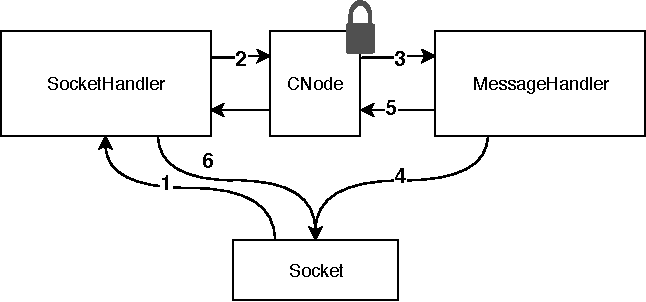
\includegraphics{Figures/dataflow}
		\caption[Overview of the message handling process in the bitcoin client.]{\label{fig:dataflow} Overview over the message handling process in the bitcoin client. This figure illustrates the flow of a message through the networking part of the bitcoin client.}
	\end{center}
\end{figure}



%\section{\label{background:scaling} Scaling issues}
%FDsets, Mutex, etc. refer to chapter on profiling





\chapter{\label{profiling}Profiling}
In this chapter, we prove that the current state of the art bitcoin client does not scale well when the number of connected nodes is increased and is therefore not well suited for the use as a relay node. First, we show general measurement on various system performance indicators. After spotting the CPU to be the possible bottleneck, we perform an in depth analysis of the runtime behaviour of the two most heavy weight threads. This leads to the insight that the inter-thread communication is the bottleneck for scaling the bitcoin client.

\begin{figure}[!hbt]
\begin{center}
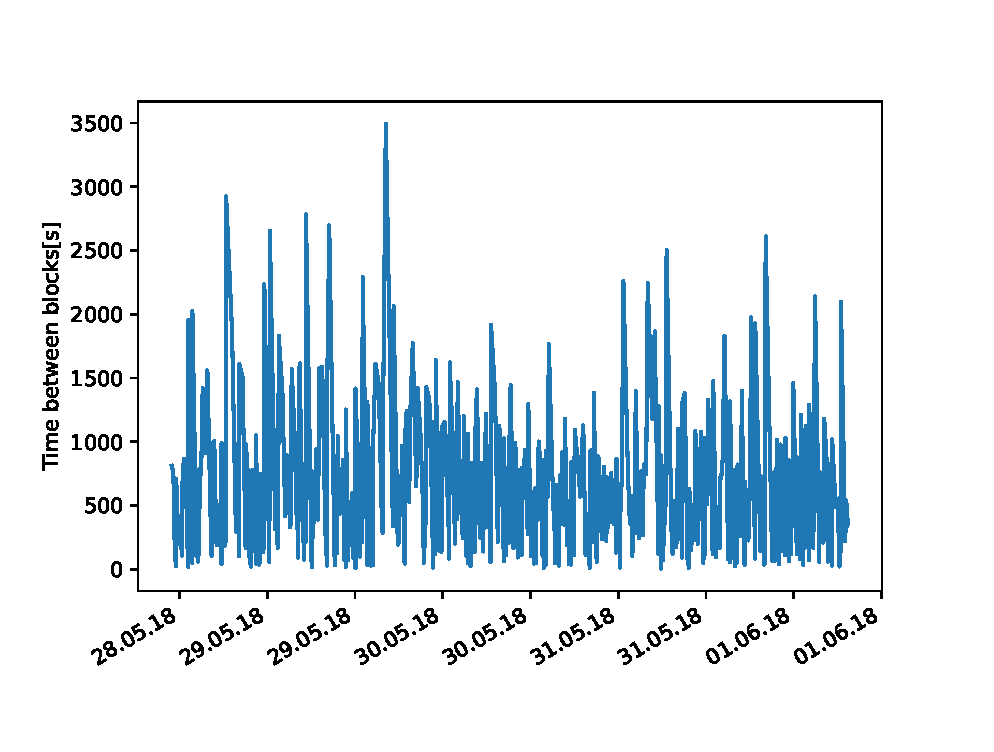
\includegraphics[width=0.5\textwidth]{block_dates}
\caption[Overview of the time between two successive bitcoin blocks.]{Overview of the time between two successive blocks. The time was measured for 650 blocks between 1.6.18 and 28.5.18 and is given in seconds on the y-axis. \label{figure:blockDates}}
\end{center}
\end{figure}

\section{Challenges \label{sec:measuringDifficutlies}}
Before we present the results, we discuss some challenges in measuring the performance of the bitcoin client. First, the bitcoin network is hard to observe in an isolated setting. The measurements were done with the bitcoin client connected to the bitcoin network. This means, that there are potentially large fluctuations in traffic. For example, as there is no fixed period for new blocks, it sometimes happens that there are no new blocks for 90 minutes. On the other hand, there are times when there are 4 new blocks in 10 minutes. To illustrate this, we plotted the time between two consecutive blocks in figure \ref{figure:blockDates}. To minimise the impact of such fluctuations, we designed the experiments to be long running and repeated them at least 3 times.\\
Second, the client does not allow an arbitrary amount of connections. The bitcoin client uses \textit{select} to query the sockets used for the connections to its peer. According to the linux manual page of \textit{select} \cite{select}, the total number of sockets that \textit{select} can handle is limited by FD\_SETSIZE which is hardcoded to 1024 on Linux distributions. Subtracting the 150 file descriptors that the client reserves for opening files and handling communication, it is possible to open 874 connections to peers. This behaviour could be changed by rewriting the logic of the bitcoin client to use \textit{poll} instead of \textit{select}, but this is not in the scope of this thesis. The consequence of this is that we were not able to generate an arbitrary load on the client during the experiments. Therefore, finding the bottleneck in the current state-of-the-art bitcoin client is hard.


\section{\label{profiling:setup}Methodology}
In this section, the general experimental setup and the tools used are presented. The actual experiments are described together with the results in section \ref{profiling:results}. 
\subsubsection{Device under test}
The experiments were run on two devices:
\begin{enumerate}
	\item Laptop with Intel dual Core i7 M620 CPU running at 2.67GHz with hyper-threading enabled. 4GB RAM. Running Debian Stretch. \newline This device is referred to as \textit{device 1}.
	\item Laptop with Intel dual Core i7 6600U CPU running at 2.60GHz with hyper-threading enabled. 20GB RAM. Running Ubuntu Xenial. \newline This device is referred to as \textit{device 2}.
\end{enumerate}
Note that \textit{device 2} has a more performant CPU and more memory than \textit{device 1}. 








\subsubsection{Client under test}
All experiments were performed with version 0.16 of the bitcoin client.\\
Only minor modifications were made to the client. First, the hardcoded connection limits were increased in net.h. 
\begin{PseudoCode}
	MAX_OUTBOUND_CONNECTIONS = 30
	MAX_ADDNODE_CONNECTIONS = 850
	DEFAULT_MAX_PEER_CONNECTIONS = 1000
\end{PseudoCode}
The values were chosen according to the limitations of the OS and the bitcoin client implementation (see section \ref{sec:measuringDifficutlies}).\\
For some experiments, it is necessary to connect two specific clients to each other. To guarantee that this connections are always established successfully, a minor change was made to always allow incoming connections from whitelisted peers. The following change was made in net.cpp:
\begin{diffCode}
@@ -1121,7 +1123,7 @@ void CConnman::AcceptConnection(const ListenSocket& hListenSocket) {
         return;
     }

-    if (nInbound >= nMaxInbound)
+    if (nInbound >= nMaxInbound && !whitelisted)
     {
         if (!AttemptToEvictConnection()) {
             // No connection to evict, disconnect the new connection
\end{diffCode}
Using the program \textit{top}, the priority of the bitcoin client process is increased to minimise the effect of background processes on the measurement.









\subsection{Measurement tools}
Various tools were used to measure the resources used by the bitcoin client. For reference, they are listed here.

\subsubsection{Ping client}
The \textit{ping client} is a modified version of the bitcoin client. This client will ignore most incoming messages and will send a bitcoin \textit{ping} message to the regular client every second. The \textit{ping client} only connects to the regular client and does not maintain or open other connections. The times when a \textit{ping} message is sent and when the \textit{pong} answers arrive are logged. Bitcoin clients by default send a \textit{ping} message every 120s. This time was reduced to one \textit{ping} per second. Note that the client does not send a \textit{ping}, if there is already a \textit{ping} request pending. Therefore, the actual period is defined as $\min\geschwungeneKlammern{1s,\mbox{RTT},\mbox{timemout}}$. The client does no other work. It does not accept other connections and does not ask for transactions or blocks. This keeps the \textit{ping client} lightweight. The exact changes can be seen in appendix \ref{appendix:pingClient}.\\
To make sure that the \textit{ping client} is able to connect to the bitcoin client, its ip was added to the whitelisted peers in the configuration of the client under test.

\subsubsection{gperftools}
\textit{gperftools}, short for great performance tools or google performance tools, was used to profile the CPU during runtime of the bitcoin client. \textit{gperftools} uses a stack sampling approach for profiling the CPU. A timer fires with a fixed frequency. When the timer fires, the profiler checks which function is currently executed by looking at the current stack frame. This approach leads to measurement inaccuracies, but it allows profiling with low overhead. The profiling time was set to multiple hours and the experiments were repeated multiple times to get statistically significant results. The exact times are given in the detailed experiment setups in section \ref{profiling:results}. \textit{gperftools} was chosen as a profiler because it is well suited for profiling multithreaded applications and produces little overhead. Note that in case of multithreaded profiling, the threads that should be profiled have to call ProfilerRegisterThread() after they are created. This will add a new timer for this thread. Configuration was done using environmental variables. The following settings were used:
\begin{PseudoCode}
	export CPUPROFILESIGNAL=12 			# signal used to start and stop profiling
	export CPUPROFILE=~/gproftools.prof 		# location to save the output profile to
	export CPUPROFILE_FREQUENCY=100 		# sampling frequency (samples/s)
	export CPUPROFILE_REALTIME=1 			# use the Linux interval timer
	export CPUPROFILE_TIMER_SIGNAL=34 		# use another timer signal not to 
							# interfer with SIGALARM
\end{PseudoCode}
\textit{gperftools} creates a profile in a binary format which can be translated to call graphs or that can be imported to kcachegrind/qcachegrind\cite{cachegrind}. These tools provide a graphical interface to navigate through the collected data. For more details, the documentation of the CPU profiler of \textit{gperftools} can be found in \cite{gperftools}.

\subsubsection{vmstat}
\textit{vmstat} is a Linux tool to report the usage of various system resources. \textit{vmstat} reads these information from the /proc filesystem. It is used, because it shows a broad overview of many system parameters such as swap usage, memory usage, disk I/O, interrupt frequency, frequency of context switches, the CPU usage and the I/O wait time. Using \textit{vmstat}, all information is in a common place which makes the analysis easier. More information can be found in the Linux manual page in \cite{vmstat}.

\subsubsection{top/ps}
\textit{top} and \textit{ps} are standard Linux tool to get realtime information about the current resource usage. They are able to show per thread CPU usage and the total amount of memory used. \textit{top} was used because of its ability to continuously measure. \textit{ps} was used because it the output can be formatted more easily, which helps for the analysis of the experiments. Otherwise, the two programs can be used interchangeably. More information about \textit{top} and \textit{ps} can be found in the Linux manual pages in \cite{top} and \cite{ps}. 




\section{\label{profiling:results}Experiments}
In this section, a series of 4 experiments is presented. First, we measure the performance of a client that is connected to an increasing numer of peers. After experiencing a performance degeneration in this experiment, a second experiment is done which shows the resource usage of the bitcoin client when it is connected to a maximum of 860 peers. The last two experiments analyse the increased CPU usage of the client and show that the inter-thread communication is limiting the scaling of the currently used standard client. In the following, the reasoning behind the experiments and the exact setups are explained and the results are presented and explained.

\begin{figure}[!bt]
\begin{center}
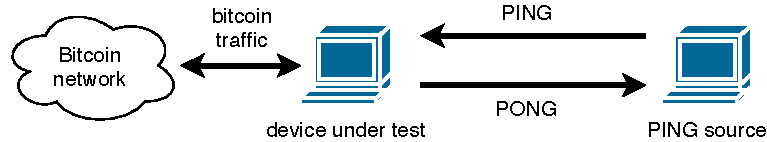
\includegraphics[width=0.8\textwidth]{Figures/pingmachine.pdf}
\caption[Test setup for the performance degeneration test]{Test setup for the performance degeneration test. The \textit{ping client} sends a \textit{ping} every second. The device under test replies with a \textit{pong} message. The times when a \textit{ping} is sent or a \textit{pong} is received are logged at the \textit{ping client}. During the test, the client receives regular bitcoin messages from its peers over the bitcoin network. \label{figure:pingmachine}}
\end{center}
\end{figure}

\subsection{Performance degeneration \label{sec:perf_degen}}
The goal of the first experiment is to show that the performance of the bitcoin client degenerates when connecting to many peers. The load on the client is dependent on the current state of the bitcoin network and the peer activity in general (see section \ref{sec:measuringDifficutlies}). Furthermore, the load is dependent on the time. For example, a higher load is expected when a block has to be verified.\\ 
There are 2 network parameters commonly measured to make assumptions about networks. The first of them is throughput. The intention would be that the bitcoin client is not able to process the data fast enough when connected to many peers and would drop packet or would throttle the amount of messages sent. As argued in section \ref{sec:measuringDifficutlies}, it was not possible to bring the client to its limits and therefore we could not observe any packet drops or intentional message throttling which makes the use of the throughput as performance indicator difficult to measure and to interpret. The other common performance indicator is the latency. We measured the RTT of a client connected to the bitcoin client under test. The expected result is an increasing delay at the client when it is connected to an increasing number of peers. To measure the performance of the client, the RTT of a \textit{ping}/\textit{pong} exchange was measured using the \textit{ping client}. According to the bitcoin protocol, upon the arrival of a \textit{ping} message, a client must respond with a \textit{pong} message\cite{bitcoinNetworkProtocol}. 
\subsubsection{Setup}
The \textit{ping client} runs on the same host as the software under test. The setup is illustrated in figure \ref{figure:pingmachine}. The experiment was conducted as follows:
\begin{itemize}
	\item The bitcoin client is started.
	\item The \textit{ping client} is started.
	\item Iterate over the following desired connection levels: 30, 100, 300, 500, 700, 860 and for each level do the following:
	\begin{itemize}
	\item Establish new connections until the desired connection level is reached.
	\item Wait for 15 minutes to assure that the client is in a steady state.
	\item The measurement starts. For 1 hour, the actual number of connected peers is logged and new connections are established, if the connection count drops below the desired level. The logged data is used to match the logs from the \textit{ping client} to a connection count level and to verify that the desired connection count matches the actual number of open connections.  
	\end{itemize}
\end{itemize}
We run the experiment 3 times on both devices. This means that every of the discrete connection levels in the experiment was measured for 3h per device.\\


\subsubsection{Results}
The results of this experiment are listed in table \ref{tab:performance_degeneration}. We are interested in the change of the measured RTT.  In figure \ref{fig:rtt}, the data is plotted. The plot shows the increase of the delay when additional connections are established at the client. We note that after 300 connections, the additional overhead per added connection gets larger. We assume that the increase is smaller for \textit{device 2}, because the device has better stats. The results show that the RTT is dependant on the number of connections which is a clear sign of bad scaling properties of the bitcoin client.\\
%Incoming messages at the client can be split into two categories: The first category contains all messages that is dependant on the number of connections, e.g. PING messages or advertisements of transactions. Messages that are independent of the number of connected peers belong to the second category. Examples for messages in this category are incoming transactions or blocks. Generally, messages of the second category cause larger overhead at the receiving client, because transactions and blocks need verification while messages from the first category can be replied without large overhead. Because of this, we would not expect the 

\begin{table}[tbp]
\begin{center}\begin{minipage}{\textwidth}
\begin{center}
\begin{tabular}{r | r |r}
\textbf{Number of connections} & \textbf{RTT \textit{device 1} [$\mu s$]} & \textbf{RTT \textit{device 1} [$\mu s$]} \\
\hline
30 & 8'198		& 3'754 \\
100 & 7'151 	& 5'630 \\
300 & 26'420 	& 8'930 \\
500 & 81'797 	& 20'794 \\
700 & 174'920 	& 30'482 \\
860 & 187'246 	& 40'246 \\
\end{tabular}
\end{center}
\end{minipage}
\caption[RTT measurements of the bitcoin client.]{RTT measurements of the bitcoin client. The RTT of a \textit{ping}/\textit{pong} exchange with the bitcoin client is measured for different numbers of peer connections.}
\label{tab:performance_degeneration}
\end{center}
\end{table}

\begin{figure}[!bt]
\begin{center}
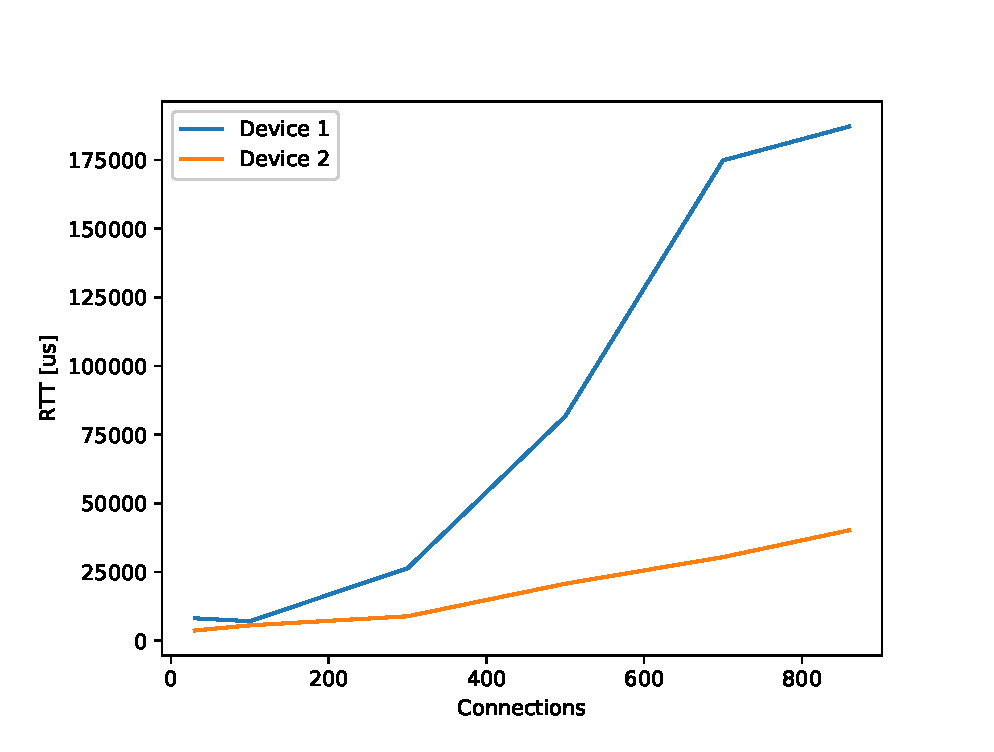
\includegraphics[width=0.7\textwidth]{rtt}
\caption[RTT measurements of the bitcoin client.]{This figure shows the measured RTT of a ping/pong message exchange when the client under test is connected to an increasing number of peers. We see that the delay is increasing with the number of connections. After around 300 connections we see a larger increase in the delay for both devices.}
\label{fig:rtt}
\end{center}
\end{figure}




\subsection{General Resource Usage \label{sec:generalResources}}
We have seen that the performance of the client becomes worse when more connections are added. To find the limiting factor on the performance, we do another experiment and measure various system parameters. CPU, I/O, Swap and Memory usage were measured. 
\subsubsection{Setup}
\begin{itemize}
	\item The bitcoin client is started.
	\item Iterate over the following desired connection levels: 30, 100, 300, 500, 700, 860. For each, do the following:
	\begin{itemize}
	\item Establish new connections until the desired connection level is reached.
	\item Wait for 15 minutes to assure that the client is in a steady state.
	\item The measurement starts. For 1 hour, the actual number of connected peers is logged and new connections are established, if the connection count drops below the desired level.\textit{vmstat} is used to measure the CPU usage in user and kernel space, the number of context switches, the I/O wait time, the amount of free memory, the amount of swap used and the amount of kernel buffer space used. One measurement is taken every 5 seconds.
	\end{itemize}
\end{itemize}
We run the experiment 3 times on both devices. This means that every of the discrete connection levels in the experiment was measured for 3h per device.\\
\subsubsection{Results}




An overview of the results can be found in table \ref{tab:recource_usage}. For the CPU measurements we note, that the CPU usage in both devices increases, while the idle time of the CPU decreases. The absolute values for the total CPU usage at 860 connections reported by \textit{vmstat} (mean value over the 3h of experiment) are 52\% and 47\% for \textit{device 1} and \textit{device 2} respectively. \textit{vmstat} gives the values in respect to the total computing power. However, it is not clear if this load is distributed evenly across the 4 virtual CPU cores both devices have. To check this, the experiment in section \ref{sec:threading} is done. \\
 We observe many context switches. Using \textit{strace}, we see that approximately 90\% of the system calls are calls to \textit{futex}. According to Franke et Al. in \cite{franke2002fuss}, the call to \textit{futex} is used for fast thread synchronisation.\\
 When looking at the I/O measurements, we note that disk reads and disk writes do not seem to be the bottleneck as the measurements at 860 nodes show a similar amount of disk reads/writes as the measurement at 30 nodes. The same is true for the I/O wait measurement which measures the time a process has to wait for I/O devices in general. We see an increase in interrupts. This is expected as the network interface does receive more messages and will therefore produce more interrupts.\\
 From the data, it is clear that swapping is not causing the performance degeneration. This is also clear as the memory usage peaks at around 35\% and there is no need for excessive swapping. Also the buffer space used to store kernel space object does not seem to run out.\\
 With these result, I/O and memory bottlenecks can be ruled out. We noted, that the CPU usage only goes up to around 50\%. Next, we will check how the workload is distributed over the cores. This will allow us to pinpoint the bottleneck to the CPU or rule this factor out as well.










\subsection{Per thread CPU usage measurement \label{sec:threading}}
We noticed that the CPU usage is increasing. However, the overall CPU usage only goes up to approximately 50\%. As the client is multithreaded, we would expect the load to spread across all 4 virtual cores. However, if the load is not distributed evenly, it could be the case that 1 or 2 cores run at 100\%. We do an additional experiment, in order to show that which part of the system is using most CPU time and that the load is not spread evenly across the cores. For this, the CPU usage was measured on a per-thread basis.\\

\subsubsection{Setup}
\begin{itemize}
	\item The bitcoin client is started.
	\item Iterate over the following desired connection levels: 30, 100, 300, 500, 700, 860. For each do the following:
	\begin{itemize}
	\item Establish new connections until the desired connection level is reached.
	\item Wait for 15 minutes to assure that the client is in a steady state.
	\item The measurement starts. For 1 hour, the actual number of connected peers is logged and new connections are established, if the connection count drops below the desired level. \textit{ps} is used with the -L command line option which shows the per thread CPU and memory usage. Measurements are taken every second.
	\end{itemize}
\end{itemize}
We run the experiment 3 times on \textit{device 1} and \textit{device 2}. This means that every of the discrete connection levels in the experiment was measured for 3h per device.\\
\subsubsection{Results}
The results of the experiment are plotted in figure \ref{fig:threads}. The result looks similar for both devices, thus only the results of \textit{device 1} are shown.
We see that the SocketHandler thread (bitcoin-net) and MessageHandler thread (bitcoin-msghand) are responsible for most of the CPU usage. At 860 connections, these two threads are using about 90\% of CPU time. Again, if the system was loaded, we would expect the CPU time for at least one of these threads to go up to 100\%.\\
The CPU time reported by top is a mean over a certain period of time. We perform a variant of the experiment with additional resolution to get a more fine grained view of the CPU usage of the SocketHandler thread and the MessageHandler thread. For this, we increase the sampling frequency and keep track of how many times the CPU time goes up to 99.9\%.
\subsubsection{Setup 2}
\begin{itemize}
	\item The bitcoin client is started.
	\item Connection setup requests are sent to the client using the command line interface. The requests are sent at a fixed frequency of 8 connections per second. During the connection establishment, the CPU usage is measured every 100ms. Additionally, the number of established connections is logged.
	\item When the client reaches 860 let it run for another minute and then stop.
\end{itemize}
The experiment was run 3 times on \textit{device 1}.\\
\subsubsection{Results 2}
 We see in figure \ref{subfigure:bursts}, that for the SocketHandler thread (bitcoin-net) the number of these "bursts" (moments when the CPU usage is above 99.9\%) of CPU usage increases with an increasing number of connections. Interestingly, we observe that starting from about 400 connections the amount of these "bursts" decreases for the MessageHandler thread at about the same rate at which it is increasing for the SocketHandler thread. The reason for this becomes clearer after the next experiment.\\


\begin{figure}[!pbt]
\begin{center}
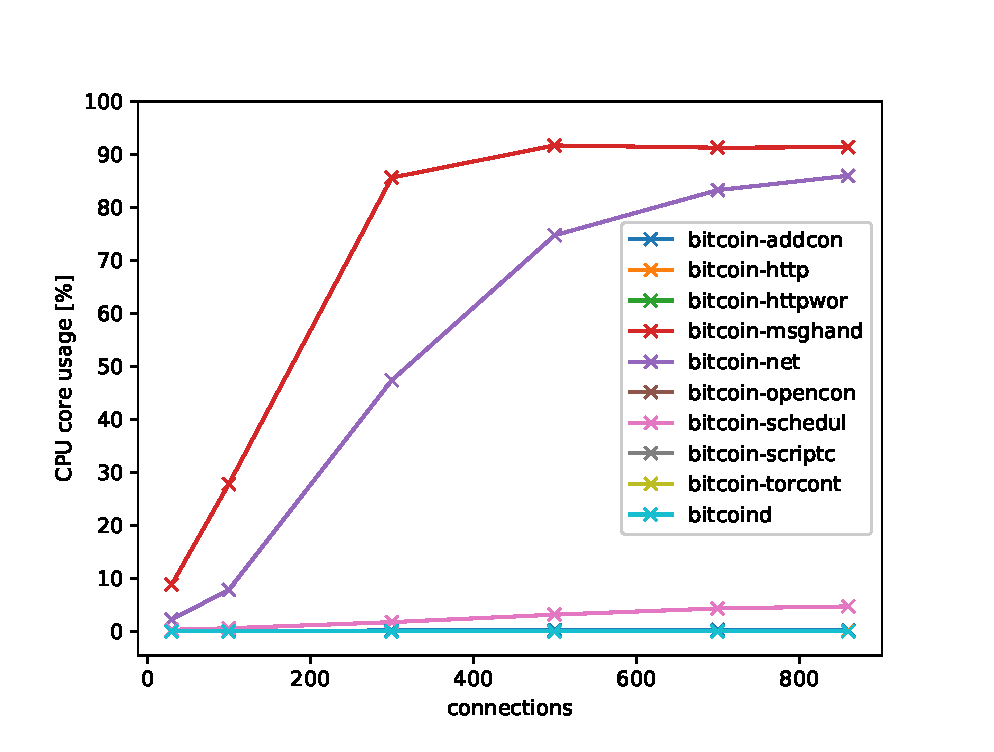
\includegraphics[width=0.7\textwidth]{threads}
\caption[Per thread CPU usage]{CPU usage of the individual threads of the bitcoin client when connected to different numbers of peers. The only two threads using a lot of CPU time are the bitcoin-net and bitcoin-msghand threads. The other threads use less than 5\% CPU time.}
\label{fig:threads}
\end{center}
\end{figure}

\begin{figure}[!pbt]
\begin{center}
\begin{subfigure}[t]{0.49\textwidth}
	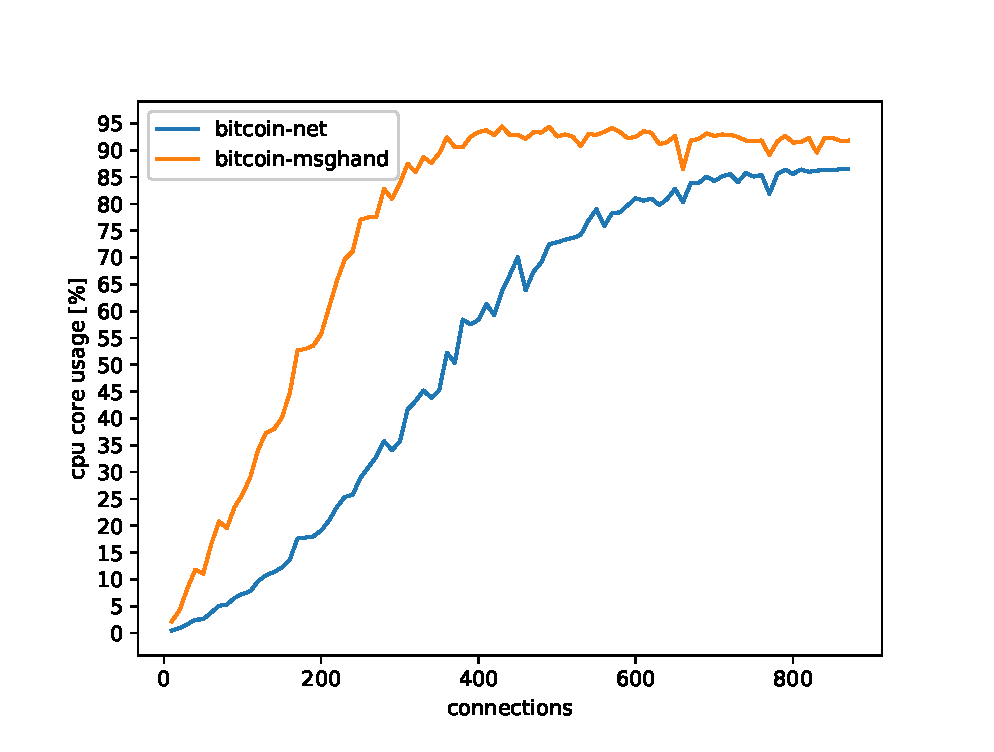
\includegraphics[width=\textwidth]{cpuUsage}
  \subcaption[CPU usage of the two most heavy weight threads.]{CPU usage of the MessageHandler and the SocketHandler as a function of the number of connected peers. We see that both threads increase to about 90\% CPU time. After that, the CPU time used does not increase anymore when adding additional connections.}
  \label{subfigure:cpuUsage}
\end{subfigure}
\hfill
\begin{subfigure}[t]{0.49\textwidth}
	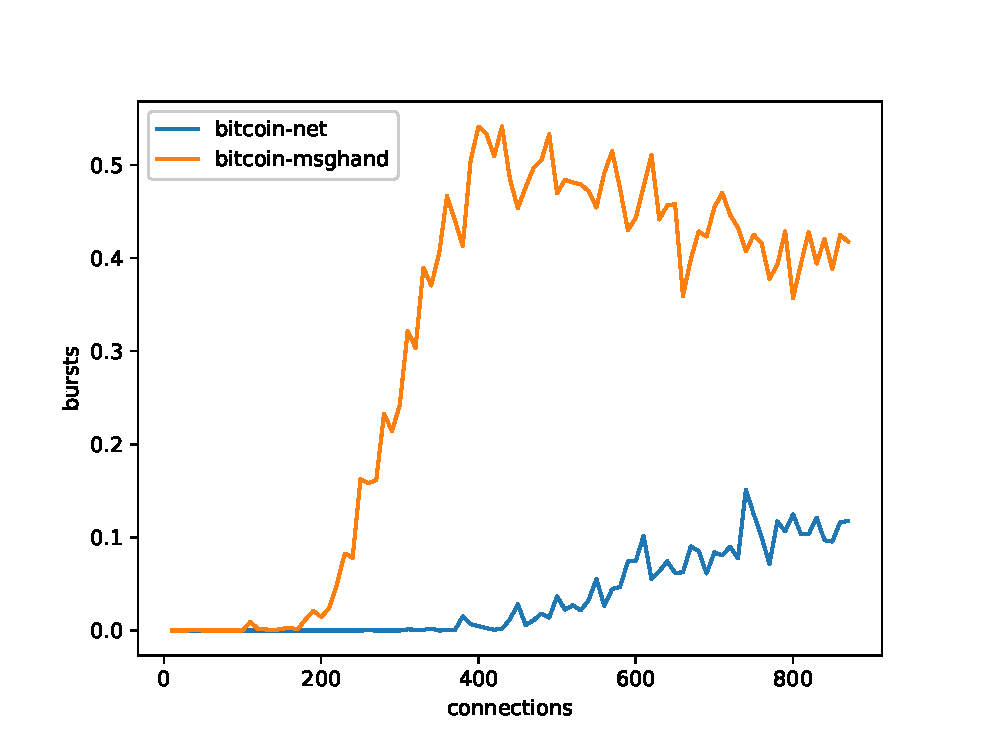
\includegraphics[width=\textwidth]{bursts}
  \subcaption{Ratio between the measurement points above and below 99.9\% CPU usage. By looking at the amount of time the threads are using more than 99.9\% CPU time, we get a more fine grained view over the trend of the CPU usage of the threads. At around 400 connections, we see that the CPU time for the bitcoin-msghand thread starts to decrease while the CPU time of the bitcoin-net thread increases.}
  \label{subfigure:bursts}
\end{subfigure}
\caption[Detailed CPU usage of the MessageHandler and the SocketHandler threads]{Detailed CPU usage of the MessageHandler and the SocketHandler threads.}
\label{fig:burst}
\end{center}
\end{figure}




\subsection{Thread work analysis \label{sec:workAnalysis}}
By now, we have strong evidence that the CPU usage is linked to the bottleneck for the scaling of the bitcoin client on our test devices.
The following experiment shows the difference in the workload distribution of the tasks that are performed by the SocketHandler thread and the MessageHandler thread under different load. 
\subsubsection{Setup}
The measurement is done using \textit{gperftools}. The experiment is conducted on \textit{device 1}. The test setup is the following:
\begin{itemize}
	\item The bitcoin client is started.
	\item Iterate over the following desired connection levels: 30, 400, 860. For each level do the following:
	\begin{itemize}
	\item Establish new connections until the desired connection level is reached.
	\item Wait 15 minutes to guarantee a normal mode of operation
	\item Profile the CPU usage using gperftools for 4 hours. For this, \textit{ProfilerRegisterThread()} was compiled in at the start of the SocketHandler thread and the MessageHandler thread to enable individual timers for these two threads.
\end{itemize}
\end{itemize}
This experiment was repeated 3 times. This leads to a total of 12h measurement for 30, 400 and 860 connections, each.

\subsubsection{SocketHandler thread}
We focus on the three function calls that use the most CPU time when 30 connections are established. Therefore, the results presented will not sum up to 100\%. An overview of these functions and what they are used for can be found below.
\begin{itemize}
	\item \textbf{\textit{CriticalBlock::CCriticalBlock}:} Wrapper that is used for thread synchronisation. Makes the current scope a critical section. A std::recursive\_mutex lock is acquired that is automatically released when the scope ends.
	\item \textbf{\textit{\_\_select}:} In the context of the bitcoin client, \textit{\_\_select} checks for incoming packets and the availability of sending messages by checking the TCP sockets of all connected clients.
	\item \textbf{\textit{CThreadInterrupt::sleep\_for}:} The calling thread waits until the timeout exceeds or the thread is waked by another thread. This roughly translates to "there is nothing to receive or send".
\end{itemize}
The result of the experiment can be seen in table \ref{tab:task_mix_socket}. Note that the time spent in \textit{CThreadInterrupt::sleep\_for} is a lot smaller at 860 connections than at 30 connections which shows that the thread has to do significantly more work. Intuitively, one would expect the \textit{\_\_select} call to grow with an increasing number of connections. Note that the results are relative numbers and only show the proportions of the function calls. This means, that the actual time spent in the \textit{\_\_select} function can be (and actually is) higher when connected to 860 peers than when connected to 30 peers, because the thread also uses more CPU time in total.\\
The main observation here is, that when connected to 860 peers, most of the CPU time used by the thread is used to handle the critical sections which are used to communicate with other threads (especially with the MessageHandler thread). 

\begin{table}[!htbp]
\begin{center}
\begin{minipage}{\textwidth}
\begin{center}
\begin{tabular}{l|r|r|r}
\textbf{Function} & \textbf{30 conn. [\%]} & \textbf{400 conn. [\%]} & \textbf{860 conn. [\%]} \\
\hline
\small CriticalBlock::CCriticalBlock & 1.7 & 38.0 & 64.9\\
\small \_\_select & 16.1 & 10.7 & 4.4 \\
\small CThreadInterrupt::sleep\_for & 80.8 & 37.5 & 3.7 \\
\end{tabular}
\end{center}
\end{minipage}
\end{center}
\caption[Difference in CPU time of 3 selected functions of the SocketHandler thread.]{Difference in CPU time of 3 selected functions of the SocketHandler thread when running with 30, 400 and 860 clients. The unit is the percentage of the cumulated CPU time of the function and all its subfunctions in respect to the total CPU time of the thread.}
\label{tab:task_mix_socket}
\end{table}



\subsubsection{MessageHandler thread}
We focus on the three function calls that use the most CPU time when 30 connections are established. Additionally, we focus on the function \textit{CriticalBlock::CCriticalBlock} because it is using a high amount of CPU time when the client is connected to 860 peers. The results do not sum up to 100\% because the some functions are filtered out. Also, \textit{CriticalBlock::CCriticalBlock} is called by various functions in the MessageHandler thread.
\begin{itemize}
	\item \textbf{\textit{PeerLogicValidation::ProcessMessages}:} This function handles the message according to the message type. This includes the verification of transactions and blocks, the request of new blocks and transactions and the assembly of responses to the peer. If possible, the messages are sent immediately.
	\item \textbf{\textit{PeerLogicValidation::SendMessages}:} Assemble messages that are not a direct response to incoming messages. This includes for example periodic \textit{ping} messages, own transactions or advertisements. If possible, the messages are sent immediately.
	\item \textbf{\textit{std::condition\_variable::wait\_until}:} The calling thread waits until the timeout exceeds or the thread is waked by another thread. This roughly translates to "there are no new messages to process".
	\item \textbf{\textit{CriticalBlock::CCriticalBlock}:} Wrapper that is used for thread synchronisation. Makes the current scope a critical section. A \textit{std::recursive\_mutex} lock is acquired that is automatically released when the scope ends.
\end{itemize}
The results of the experiment are summarized in table \ref{tab:task_mix_message}. As expected, the functions \textit{PeerLogicValidation::SendMessages} and \textit{PeerLogicValidation::ProcessMessages} increase with the number of connections. This is because more connections lead to more incoming and outgoing messages. From the decrease of \textit{std::condition\_variable::wait\_until}, we see that the thread spends less time idle. Like with the SocketHandler thread, we observe a clear increase of the overhead of thread synchronising tasks. This increase seems to be lower after 400 connections.

% also mention last experiment

\begin{table}[htbp]
\begin{center}
\begin{minipage}{\textwidth}
\begin{center}
\begin{tabular}{l|r|r|r}
\textbf{Function} & \textbf{30 conn. [\%]} & \textbf{400 conn. [\%]} & \textbf{860 conn. [\%]} \\
\hline
\small PeerLogicValidation::ProcessMessages 	& 2.6  & 20.5  	& 31.4\\
\small PeerLogicValidation::SendMessages 		& 8.5  & 66.7	& 66.3 \\
\small std::condition\_variable::wait\_until 	& 88.7 & 10.4	& 1.3 \\
\hline
\small CriticalBlock::CCriticalBlock 			& 1.5 & 30.3 	& 36.5 \\
\end{tabular}
\end{center}
\end{minipage}
\end{center}
\caption[Difference in CPU time of 4 selected functions of the MessageHandler thread.]{Difference in CPU time of 4 selected functions of the MessageHandler thread when running with 30, 400 and 860 clients. Note that the function \textit{CriticalBlock::CCriticalBlock} is not entirely called directly by the main routine of the thread but also include calls from subfunctions of the main routine of the thread. The unit is the percentage of the cumulated CPU time of the function and all its subfunctions in respect to the total computation time of the thread.}
\label{tab:task_mix_message}
\end{table}


\subsubsection{Interpretation}
From the data we collected we can see the following: 
First, we see that both heavy weight threads (MessageHandler and SocketHandler thread) spend less time idle while both coming near the limit of 100\% CPU core time. 
Second, we see that both threads use an increasing amount of CPU time for handling the acquiring and freeing of mutex locks. The current implementation of the bitcoin client uses recursive mutexes from the standard library to protect shared resources. Gautham et al. show in \cite{gautham2012implications} that the use of mutexes does not scale when handling many small critical sections. The current implementation of the bitcoin client writes every message into a CNode at least once which will lead to an increasing amount of lock/unlock operations when the number of connections is increased. 
The next observation is that for the MessageHandler thread, the amount of time spent in CriticalBlock::CCriticalBlock is almost stagnant between 400 connections and 860 connections. At the same time, we observed in the experiment in section \ref{sec:threading} that the CPU usage for the MessageHandler decreases after 400 connections. Together, these two observations lead us to the conclusion that CPU usage is not the bottleneck of the scaling of the bitcoin client, but the inter-thread communication. The increased amount of context switches due to calls to \textit{futex} that we have observed in section \ref{sec:generalResources} supports this hypothesis.


%\begin{table}[htbp]
%\begin{center}
%\begin{minipage}{\textwidth}
%\begin{center}
%\begin{tabular}{l|l|r|r|r|r|r|r }
%\textbf{category} & \textbf{Parameter} & \textbf{30} & \textbf{100} & \textbf{300} & \textbf{500} & \textbf{700} & \textbf{860} \\
%\hline
%CPU    & User & 100 & 191 & 555 & 689 & 726 & 743\\
%       & Sys & 100 & 151 & 442 & 666 & 718 & 742\\
%   & Idle & 100 & 94 & 66 & 55 & 53 & 52 \\
%   & Context switches & 100 & 316 & 2507 & 3934 & 4145 & 4195 \\
%\hline
%I/O    & Interrupts & 100 & 134 & 319 & 447 & 522 & 571 \\
%   & Disk reads & 100 & 40 & 31 & 40 & 97 & 89\\
%   & Disk writes & 100 & 40 & 48 & 55 & 61 & 65\\
%   & I/O wait & 100 & 45 & 35 & 39 & 49 & 46 \\
%\hline
%Swap & Swap & 100 & 100 & 100 & 100 & 100 & 100\\
%\hline
%Memory & Free memory & 100 & 100 & 200 & 241 & 277 & 408\\
%   & used Buffer space & 100 & 100 & 69 & 54 & 34 & 44\\
%\end{tabular}
%\subcaption{Results of \textit{device 1}}
%\vspace{5mm}
%\end{center}
%\end{minipage}
%\begin{minipage}{\textwidth}
%\begin{center}
%\begin{tabular}{l|l|r|r|r|r|r|r }
%\textbf{category} & \textbf{Parameter} & \textbf{30} & \textbf{100} & \textbf{300} & \textbf{500} & \textbf{700} & \textbf{860} \\
%\hline
%CPU    & User & 100 & 168 & 320 & 417 & 449 & 456\\
%       & Sys & 100 & 147 & 290 & 497 & 624 & 659\\
%   & Idle & 100 & 94 & 77 & 66 & 61 & 60 \\
%   & Context switches & 100 & 460 & 5208 & 10355 & 12817 & 13247 \\
%\hline
%I/O    & Interrupts & 100 & 161 & 736 & 1346 & 1679 & 1779 \\
%   & Disk reads & 100 & 32 & 2856 & 146 & 122 & 174\\
%   & Disk writes & 100 & 84 & 131 & 180 & 220 & 261\\
%   & I/O wait   & 100 & 100     & 100     & 100     & 100     & 100\\
%\hline
%Swap & Swap & 100 & 100     & 100     & 100     & 100     & 100 \\
%\hline
%Memory & Free memory & 100 & 82 & 66 & 51 & 37 & 32\\
%   & used Buffer space & 100  &  100 &   100  &  100 & 98 & 83\\
%\end{tabular}
%\subcaption{Results of \textit{device 2}}
%\end{center}
%\end{minipage}
%\caption{Resource usage measurement on both test devices for 6 connection count levels which were each measured for 3 hours. The numbers are given as percentage in respect to experiment with 30 connections to be able to better compare the results from both devices.}
%\label{tab:recource_usage}
%\end{center}
%\end{table}

\begin{table}[tbp]
\begin{center}	
\begin{minipage}{\textwidth}
\begin{center}
\begin{tabular}{l|l|l|r|r|r|r|r|r }
\textbf{Category} & \textbf{Parameter} & \textbf{Unit} & \textbf{30} & \textbf{100} & \textbf{300} & \textbf{500} & \textbf{700} & \textbf{860} \\
\hline
CPU & User & \%             & 7.35 & 12.83      & 34.40     & 41.34     & 43.20     & 43.84 \\
    & Sys  & \%             & 1.18 & 1.77       & 5.24  & 7.73      & 8.29      & 8.55 \\
    & Idle & \%             & 90.29 & 84.82         & 59.77 & 50.37         & 47.86         & 47.02 \\
    & Context switches & /5s  & 3'012.09 & 9'542.94 & 75'166 & 115'066  & 121'064   & 122'702 \\
\hline
I/O & Interrupts & /5s       & 1'117.95     & 1'492.87  & 3'538.71  & 4'913.56  & 5'702.34  & 6'187.21 \\
    & Disk reads   & /5s     & 409.73   & 154.80    & 124.67    & 157.03    & 412.13        & 386.02 \\
    & Disk writes   & /5s    & 554.82   & 208.19    & 245.07    & 279.40    & 309.36    & 336.65 \\
    & I/O wait     & s/5s       & 1.09      & 0.48      & 0.38      & 0.42      & 0.53      & 0.51 \\
\hline
Swap & Swap   & KB          & 327'516 & 327'656 & 327'992 & 328'202 & 328'595 & 327'470 \\
\hline
Memory & Free memory  & KB          & 133'188 & 132'763 & 259'472 & 314'197 & 357'951 & 540'859 \\
       & used Buffer space  & KB    & 108'994 & 107'321 & 69'476.4 & 52'858 & 39'889.5 & 45'220.6 \\
\end{tabular}
\subcaption{Results of \textit{device 1}}
\vspace{5mm}
\end{center}
\end{minipage}
\begin{minipage}{\textwidth}
\begin{center}
\begin{tabular}{l|l|l|r|r|r|r|r|r }
\textbf{Category} & \textbf{Parameter} & \textbf{Unit} & \textbf{30} & \textbf{100} & \textbf{300} & \textbf{500} & \textbf{700} & \textbf{860} \\
\hline
CPU & User &\%              & 9.30 		& 14.03 		& 25.74 		& 32.33 		& 34.71 		& 35.18 \\
    & Sys  &\%             & 2.08 		& 2.82 		& 5.57 		& 9.00 		& 11.22 		& 11.75 \\
    & Idle &\%             & 88.24 	& 82.78 		& 68.3 		& 58.33 		& 53.75 		& 52.74 \\
    & Context switches &/5s & 2'719.2 	& 11'265.9 	& 124'961 	& 234'297 	& 290'314 	& 298'712 \\
\hline
I/O & Interrupts &/5s       & 904.87 	& 1'363.25 	& 5'665.1 	& 9'719.25	& 12'199.8 	& 12'916.9 \\
    & Disk reads &/5s       & 221.15 	& 1.31 		& 12.75 		& 7.05		& 3.51		& 3.80 \\
    & Disk writes &/5s      & 340.51 	& 84.01 		& 129.41 	& 175.03 	& 218.09		& 245.50 \\
    & I/O wait &s/5s         & 0.39 		& 0.33 		& 0.33 		& 0.33 		& 0.33		& 0.33 \\
\hline
Swap & Swap &KB            & 256 & 256 & 256 & 256 & 256 & 256 \\
\hline
Memory & Free memory &KB           & 1938250 & 1758470 & 1355480 & 890892 & 324599 & 204854 \\
       & used Buffer space &KB      & 2'293.33 & 2'293.33 & 2'293.33 & 2'293.33 & 2'148.7 & 1'565.18 \\
\end{tabular}
\subcaption{Results of \textit{device 2}}
\end{center}
\end{minipage}
\caption[General resource measurements of the bitcoin client.]{Resource usage measurement on both test devices for 6 connection count levels which were each measured for 3 hours.}
\label{tab:recource_usage}
\end{center}
\end{table}











\section{Conclusion}
It was shown that the current bitcoin client does not scale well when adding additional connections. In this section, the most important drawbacks of the official bitcoin client are listed.
\begin{itemize}
	\item Thread synchronization: In the experiments that were conducted in sections \ref{sec:generalResources} and \ref{sec:workAnalysis} it was shown that thread synchronization is the largest obstacle for scaling the client to support multiple thousands of connections. Another design with less inter-thread communication should be used to improve scalability.
	\item FD\_SET: The use of select in the client limits the current maximum number of connections to 874. To be able to scale, the client should use another mechanism to handle more connections.
	\item Per connection state: The current implementation stores a considerable amount of memory in the CNodes. To be able to support large numbers of connections, the per connection state should be reduced to reduce the overall memory consumption.
\end{itemize}
To resolve these shortcomings of the current bitcoin client will be the design goal of the proposed framework in chapter \ref{design}.









%** Design.tex: How was the problem attacked, what was the design
%               the architecture 
\chapter{\label{design}Design}
We have seen, that the current bitcoin client does not scale well because of its inter-thread communication. While there are different approaches to speed up or eliminate inter-thread communication, we propose a different solution to the problem. We reduce the tasks of the relay to the bare minimum. The sole purpose of the new client should be to relay blocks. We propose to have a special programmable switch which acts as a block cache. A special firmware is able to translate requests into local lookups. A separate controller hosts the more sophisticated part of the logic, like validating blocks. This controller is responsible for updating the switch with new blocks upon their arrival and informs connected peers about the new block. The design uses UDP as the underlaying transport protocol. The benefit of this is, that due to its stateless nature, a UDP based protocol is able to scale better. As much work as possible is handled in hardware. This framework is called SABRE and is the design of M.Apostolaki and the Networked Systems Group at ETH Zürich \cite{apostolaki2018}.\\
We solve all scaling problems of the current bitcoin client noted in chapter \ref{profiling}: Only one client is effectively connected to the controller at a given time. Therefore, we see from the measurements in chapter \ref{profiling} that we do not expect a large communication overhead. All other clients are able to request the blocks at line rate from the switch. Because the switch has a clearly defined response to a request, there is no need for inter-thread communication. Therefore there is no scaling problem of the inter-thread communication at the switch as well. The controller is able to handle a theoretical unlimited amount of connections while using only one single socket for the connection to the switch. This solves the limited socket problem that is imposed by the use of FD\_SET. As we will show in the evaluation in chapter \ref{evaluation}, the design also uses considerably less memory per connection.\\
This thesis focuses on the modifications that are necessary on the clients and the controller. In this chapter, the message protocol is presented in \ref{sec:functional_overview}. The design of the client and the controller is presented in sections \ref{sec:design:design}. The chapter is concluded with a discussion of the shortcomings of the current design in section \ref{sec:design:shortcomings}.


\section{Terminology}
The design in this chapter and the following evaluation in chapter \ref{evaluation} use 3 different bitcoin clients. To avoid misconceptions, they are briefly explained here. For a more throughout explanation of the modified clients, see sections \ref{design:modifiedBitcoinClient} and \ref{design:SwitchController}. Also, a few other commonly used terms are defined here.
\subsubsection{Regular Bitcoin Client}
The term \textit{bitcoin client} is used for the unmodified bitcoin client from the official repository on GitHub \cite{bitcoinRepo}. Version 0.16 (commit bf3353de90598f08a68d966c50b57ceaeb5b5d96) was used throughout this work. We use the term \textit{regular} when referring to the unmodified bitcoin client or the unmodified bitcoin protocol.
\subsubsection{Modified Bitcoin Client}
The \textit{modified bitcoin client} is based on the \textit{bitcoin client} and is augmented with additional features. This allows the modified bitcoin client to connect to the switch relay. The modified bitcoin client can be used as a drop-in replacement for the bitcoin client.
\subsubsection{Controller}
The \textit{controller} is based on the \textit{bitcoin client} and is augmented with additional features. It is used to interface with the p4 switch and to modify its state. This code is not intended to run on a regular bitcoin node.
\subsubsection{Network protocol}
We refer to the regular bitcoin peer-to-peer network as the \textit{network protocol}. 
\subsubsection{Relay protocol}
We name the here presented addition to the communication logic \textit{relay protocol}, as it differs completely from the \textit{network protocol}.




\begin{figure}[bt]
  \begin{center}
	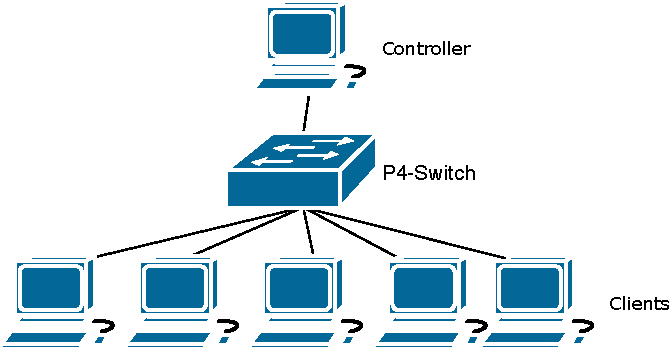
\includegraphics[width=0.5\textwidth]{Figures/DesignOverview}
  \caption{Overview of the different participants of the relay protocol.}
  \label{fig:setup:overview}
  \end{center}
\end{figure}

\section{Protocol overview \label{sec:functional_overview}}
The protocol that is presented here, differentiates among 3 parties. An overview can be found in figure \ref{fig:setup:overview}. The first group consists of the clients. We assume there to be many clients. The clients have 2 goals. They want to receive new blocks and they want to redistribute blocks that they have learned about. The second group consists of the switch. The switch is a piece of programmable hardware. It acts as a cache. Answers to a predefined set of requests can be delivered at line rate. The last protocol participant is the \textit{controller}. The \textit{controller} is used to handle uncacheable requests and to do the more sophisticated computation. It is also responsible for writing the data to the switch.\\
The protocol that connects these 3 groups is now presented. The design of the system and the network was done by M.Apostolaki and the Networked Systems group at ETH Zürich.\\
The protocol can roughly be split into 3 parts which are illustrated in figure \ref{figure:messagingProtocol}. Unless otherwise stated, UDP datagrams are used as underlaying transport protocol. The first part of the protocol (see figure \ref{figure:handshake}) handles the connection setup between the client and the switch. A 3-way handshake is used to establish the connection. The client initiates a handshake. After receiving the handshake request, the switch replies with a message containing a secret value. To complete the handshake, the client sends another message containing the same secret back to the switch. The secret is used to protect the switch from spoofing. After the handshake is complete, a message containing the connection details of the client is sent to the controller to store this metadata.\\
The second part of the protocol (figure \ref{figure:upd}) handles the update process of the switch. When a \textit{modified bitcoin client}, which is connected to the switch, receives a new block, it advertises it to the switch. If the switch does not know this block, it will tell the client to connect to the controller at a specified port/IP. This connection is established using the regular bitcoin protocol. After the client has connected to the controller, it will send the new block to the controller. After that, the connection is closed and the controller updates the switch. It will first send a message indicating, that a new block will be sent. After that, the block is sent in chunks of 499 bytes to the switch. These block fragments are called segments. The last segment is padded to have the same size. This is needed because of limitations of the switch. A precomputed UDP checksum is added, to reduce the computation that the switch has to do on an incoming request.\\
After the controller updated the switch, it will advertise the new block to all connected clients. Part 3 (figure \ref{figure:inv}) of the protocol explains how blocks are distributed to the clients. The controller sends an advertisement containing the hash of the block and the total number of segments, the block was split into. The clients that are interested in the block can request the individual segments from the switch directly. From this point on, the controller does not have to do any more work for distributing this block. A client has to request all segments seperately to be able to reconstruct the block.


\subsection{Message types \label{sec:messagingProtocol}}
The \textit{relay protocol} uses a set of message types for the communication between client, switch and controller. The message types and their use are listed here for reference. To see, in which part of the protocol the messages are used, see figure \ref{figure:messagingProtocol} The focus lays on the functional aspects of the message types. The exact message structures and sizes are listed in appendix \ref{appendixMessagingProtocol}. For better readability, the message types of the \textit{relay protocol} are written using capital letters throughout this thesis.
\begin{itemize}
	\item REY: This message type is used to establish a connection between the client and the switch. A 3-way handshake is performed. The messages of the individual steps of this handshake are marked using a flag.
	\item INV: The INV message is used by the controller to advertise new blocks. It contains the block hash and the number of segments the block is split into.
	\item SEG: Using the SEG message, the client requests a segment of a block from the switch. For this, the message contains the hash of the block and the segment number that is requested.
	\item BLK: The BLK message is used by the controller to update the switch. The message contains the segment ID and the data. Additionally, the packet contains a precomputed checksum which is used by the switch to create the UDP checksum when the client requests the block. Note that the UDP checksum depends on the destination port and can therefore not be computed in advance and must be calculated by the switch. \\ The switch sends BLK messages as reply to SEG messages from the client. These BLK messages only contain the segment ID and the data.
	\item ADV: The client sends an ADV message to the switch to indicate that it received a new block. This message contains the hash of the new block.
	\item CTR: The switch may respond to an ADV message with a CTR message, indicating that the client should connect to the controller. The message contains the IP and the port which should be used to connect to the controller.
	\item UPD: The UPD message is sent by the controller. The switch uses this message as an indicator, that the controller wants to add a new block. The message contains the hash of the new block.
	\item BCL: The BCL message is used to blacklist a peer and is sent from the client to the switch.
	\item CON: After a successful handshake with a new client, the switch sends a CON message with IP and port of the client to the controller. This message is used to inform the controller about new connections.
\end{itemize}




\begin{figure}[!bt]
\begin{center}
\begin{subfigure}[b]{0.32\textwidth}
	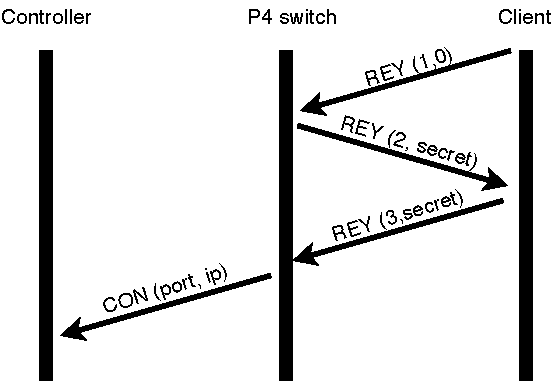
\includegraphics[width=\textwidth]{Figures/Handshake.pdf}
  \subcaption{Handshake}
  \label{figure:handshake}
\end{subfigure}
\begin{subfigure}[b]{0.32\textwidth}
	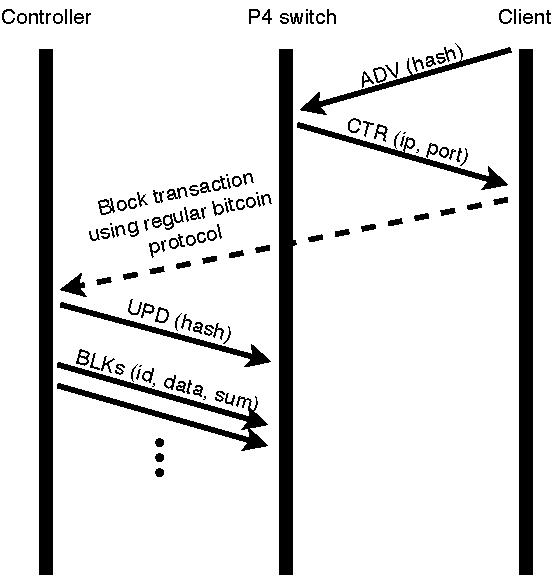
\includegraphics[width=\textwidth]{Figures/UPD.pdf}
  \subcaption{switch update}
  \label{figure:upd}
\end{subfigure}
\begin{subfigure}[b]{0.32\textwidth}
	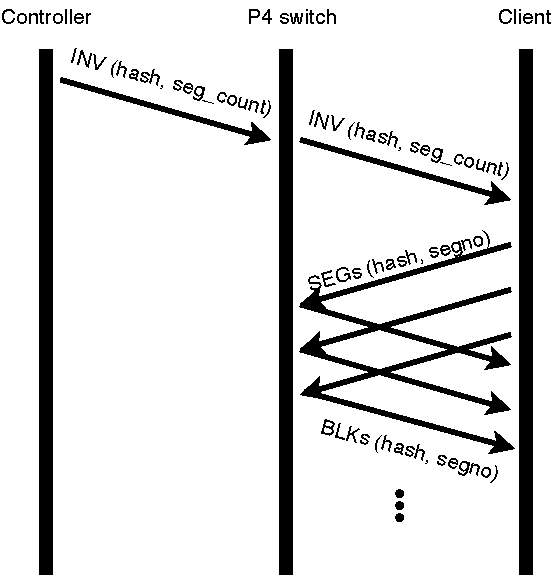
\includegraphics[width=\textwidth]{Figures/INV.pdf}
  \subcaption{client side block request}
  \label{figure:inv}
\end{subfigure}
\caption[Overview of the individual phases of the relay protocol.]{Overview of the individual phases of the \textit{relay protocol}.}
\label{figure:messagingProtocol}
\end{center}
\end{figure}




\section{Client and Controller Implementation  \label{sec:design:design}}
The changes to the bitcoin client aim at being lightweight and modular. First, we describe some general design choices that are common to both the \textit{modified client} and the \textit{controller}. Next, we discuss the peculiarities of the \textit{modified client} and the \textit{controller}.\\
The full implementation can be found in \cite{bitcoinFork}.

\subsection{General design}
Both, the \textit{modified client} and the \textit{controller} are based on the \textit{regular bitcoin client}. The benefit of this is, that parts of the existing code can be reused. One decision in the design process was to have most of the logic inside a separate C++ class to be able to quickly get an overview of the additional logic.\\
For better testability of the design, the 3 software types, namely the \textit{regular client}, the \textit{regular bitcoin client} and the \textit{controller} can be chosen at startup without the need to recompile. This results in a minimally larger binary compared to an approach where the type has to be specified at compile time. Besides the client type, other new command line or config file parameters were introduced. They allow to set the IP address and the port of the switch, as well as the own port that is used to connect to the relay. \\
Thanks to the socket abstraction, the logic for incoming messages can be reused. After a packet is read from the socket, the code checks if it is coming from the switch. If this is the case, it is handed over to the relay network message handler instead of the normal message handler. For sending, the handler checks if the outgoing message should use UDP before sending because the logic for sending is slightly different between TCP and UDP. Since UDP is connection-less the sender has to provide the destination IP and port.\\

\subsection{Modified Bitcoin Client \label{design:modifiedBitcoinClient}}
The modified client runs on a users device. Along the regular tasks of a regular bitcoin client, the modified client also fulfills the here mentioned tasks.
\subsubsection{Connection setup}
When the modified client starts its networking routine, a Net\_relay object is generated. This object is handles the logic that is used to interface with the switch. A new UDP port is created with the connection settings found in the settings. Using the command line or the config file, the default settings for ip address and port of the switch can be overwritten. In a productive setting, anycast could be used to find a relay switch. \\
The CNode construct of the unmodified bitcoin client was used to enhance the integration with the existing codebase. This allows, for example, to get a report over the connected switch using bitcoin-cli as it is possible with regular connections. To be able to differentiate between the UDP connection used for the switch and the TCP connections of regular peers, a isRelay flag was added to the CNode class.\\
After the CNode is created, the client tries to establish a connection to the switch. As long as the client is not connected to the switch, every minute, a handshake is initiated by sending a REY message. The switch will answer with another REY message containing a secret. Using the same secret, the 3-way handshake is concluded. After the handshake, the relay connection will go to a connected state which will activate all other switch specific functionalities.\\
The fact that the same data structure could be used for the connection to the relay and for peer connections, means that the relay connection does not introduce more memory overhead than a regular peer connection. Furthermore, because the relay connection uses UDP instead of TCP, less state has to be maintained in kernel space. 


\subsubsection{Incoming message handling}
The bitcoin client checks for incoming messages using FD\_SETs. Because of the socket abstraction, the same mechanism as for checking the other connections can be used. The distinction begins when the data is received. A separate handler is responsible for the arrival of messages from the switch. The new code was not included in the main message handling routine, because the message format is completely different and this way, the code for both connection types is logically separated. \\
\textbf{INV messages:} An incoming INV message is first translated into an inv message from the \textit{regular bitcoin protocol}. This allows us to reuse the checks that are done on regular messages. These checks tell, if the client is interested in this block or will ignore the message. \newline
If the client does want the block, it is requested from the switch. A small data structure is created which holds the hash and the number of segments and the segments themselves. Two timestamps are added which are used to check the soft and hard timeout of the segments. Using these timestamps, a timeout handler for the block is implemented as can be seen in figure \ref{pseudocode:timeoutHandler}. All segments are then requested from the switch. A small delay of 1ms between the SEG messages is introduced, which leads to a drastically lower packet loss rate because of less congestion at the switch. Because the switch is emulated in software, it is not able to process the requests at line rate and starts to drop packets if they arrive in too fast succession. \\
\textbf{BLK messages:} When a BLK message arrives, it is checked if the containing segment belongs to a block that the client requested from the switch. If it does, it is added to the list of arrived segments. As soon as the block is completed, it is given to the MessageHandler thread to be processed. From this point, the logic is the same as if the block was received over the regular bitcoin network. \\
\textbf{CTR messages:} An incoming CTR message means, that a connection to the controller should be established. The already existing mechanism for connecting to a peer can be reused. A flag indicating that the new connection is a "manual connection" is added to the function call to make sure that the client connects to the controller.\\  
The other message types are ignored on the client and are silently dumped.



\begin{figure}[tb]
	\begin{center}
		\begin{PseudoCode}
while(not all segments received):
	if(time since last segment > timeout threshold):
		request retransmission of all non yet arrived segments
	else:
		request retransmission of all blocks with id < latest segment - 10
	wait 1s
\end{PseudoCode}
\caption[Pseudocode for the segment timeout handler]{\label{pseudocode:timeoutHandler}Pseudocode for the segment timeout handler. The handler uses a sliding window to trigger the retransmission of lost segments.}
	\end{center}
\end{figure}






\subsection{Switch Controller\label{design:SwitchController}}
The controller is a \textit{regular bitcoin client} which has the extra task to manage updates of the switch and to advertise new blocks. The decision to design the controller as an addition to the regular bitcoin client is based on the fact that the block validation logic can be reused. This way we make sure that the switch is updated with legitimate blocks and is not updated with arbitrary data. Otherwise, the setup could be used by a malicious user as free anonymous cloud disk space which he could fill with malicious or illegal data.\\
The controller receives CON messages, when a new client successfully connects to the switch. A CON message contains the IP address and the port of the client. This metadata needs to be stored. The std::set data structure was chosen, as it offers a complexity of $O(\log(n))$ for lookup and insert.\\
If a new client connects to the controller, client and controller use the regular bitcoin protocol to exchange blocks and transactions. The goal of this connection is for the controller to learn a new block. When the controller received the block from the client, the connection is closed by the controller. The connection is also closed after a timeout of 120s.\\
After a new block is received that can be attached to the longest chain, the switch has to be updated. For this, the controller sends an UPD message, followed by the block. According to the messaging protocol, the block has to be sent in segment with 499 bytes of data each. The last segment is padded to have a 499 byte length as well. The switch needs a precomputed UDP checksum to be able to send BLK responses to SEG requests by the client. At this point, the final checksum cannot be calculated, as the port of the client is part of the checksum. Figure \ref{code:udpchecksum} shows the pseudo code for creating the precalculated UDP checksum. The protocol does not specify an answer to the update process of the switch. This means that the controller does not get any feedback if the update was successful or not. During the evaluation of the setup using mininet, we observed that the switch drops packets if they arrive in fast successive bursts. Therefore, the current controller will immediately send a fragment as soon as it is ready and not first queue it and let it send by the SocketHandler thread. Additionally, while sending, a 1ms delay was added between two successive segments. It is not clear, if the delay is needed or would have to be adapted in a real world scenario with actual hardware.\\
After the switch is updated, the controller advertises the block to all clients for which it has an entry in the connection metadata set.


\begin{figure}[tb]
\begin{center}
	\begin{PseudoCode}
udpPreChecksum(bytes):
    // Calculate the sum
    sum = 0;
    len = len(bytes)
    
    // sum up the 16 bit values
    for(i=0; i<len/2; len+=2):
        sum += bytes[i]<<8 + bytes[i+1];
        if (sum & 0x80000000):
            sum = (sum & 0xFFFF) + (sum >> 16);

    // Add padding if the packet length is odd
    if ( len & 1 ):
        sum += bytes[len-1];

    // Add the pseudo-header
    sum += IPPROTO_UDP;
    sum += length + 8;
    sum += length + 8;

    // Add the carries
    while (sum >> 16):
        sum = (sum & 0xFFFF) + (sum >> 16);

    return sum;
	\end{PseudoCode}
	\caption[Pseudocode of the precalculated UDP checksum]{Pseudocode of the precalculated UDP checksum. \label{code:udpchecksum}}
	\end{center}
\end{figure}





\section{Design shortcomings \label{sec:design:shortcomings}}
In this section, some shortcomings of the design are discussed. Part of them is due to limitations of the \textit{relay protocol} (see section \ref{sec:messagingProtocol}) and some are due to the fact that the current design is a prototype. 
\subsubsection{Missing error handling}
If for some reason, a packet is dropped during the update of a switch, the update is not successful. However, the controller does currently not know that the update was not successful. It sends out INV messages but the clients receiving the INV messages will not be able to correctly reconstruct the block from the segments. To tackle this, the switch should implement some feedback on the update process such as the number of segments received and it should check if it receives all segment ids.
\subsubsection{Increasing state}
The current implementation of the \textit{controller} does not specify a timeout after which the metadata about the connected clients should be deleted. This means that there is a protocol based attack vector. It is possible to fill up the free memory of the controller by performing handshakes with the switch using a large amount of possible IP addresses and port pairs. While the switch offers DOS protection, the attack is still successful if it is performed over a large timespan. To protect against this, the controller should implement a maximum lifetime of the client entries that it stores. Another possibility would be to create a list of fixed length and to remove the oldest entries if a new client connects. Currently, the information about the clients is never removed.
\subsubsection{Multiple block update}
Currently, only the update of a single block is supported. This means, that when a client which has multiple new blocks connects to the \textit{controller}, only the newest one is sent to the switch. This is of course not practical for a real world deployment. This behaviour can easily be changed as soon as the switch supports multiple blocks.
\subsubsection{Windows and IPv6 support}
The prototype was tested on Linux and on MacOS. It was not tested if it runs on windows hosts. The current \textit{relay protocol} does not have support for IPv6 addresses which are therefore not supported by the client.
































%** Results.tex: What were the results achieved including an evaluation
%
\chapter{Evaluation \label{evaluation}}
The implementation of the modified client and the controller was tested using mininet. The evaluation focuses on the modified client and the controller which are the results of this thesis. The software for the switch was written by M.Apostolaki from ETH Zürich.\\
The evaluation starts with a general setup in \ref{evaluation:setup}. This shows that the protocol is working as expected. Additionally, we measure the speed of the block distribution. After analysing the scaling properties of the protocol in section \ref{evaluation:scaling} and comparing the message sizes of the proposed solution to the state-of-the-art bitcoin client in \ref{evaluation:messages}, we measure the memory and CPU overhead in sections \ref{evaluation:memory} and \ref{evaluation:cpu} respectively.

\begin{figure}[!hbt]
  \begin{center}
	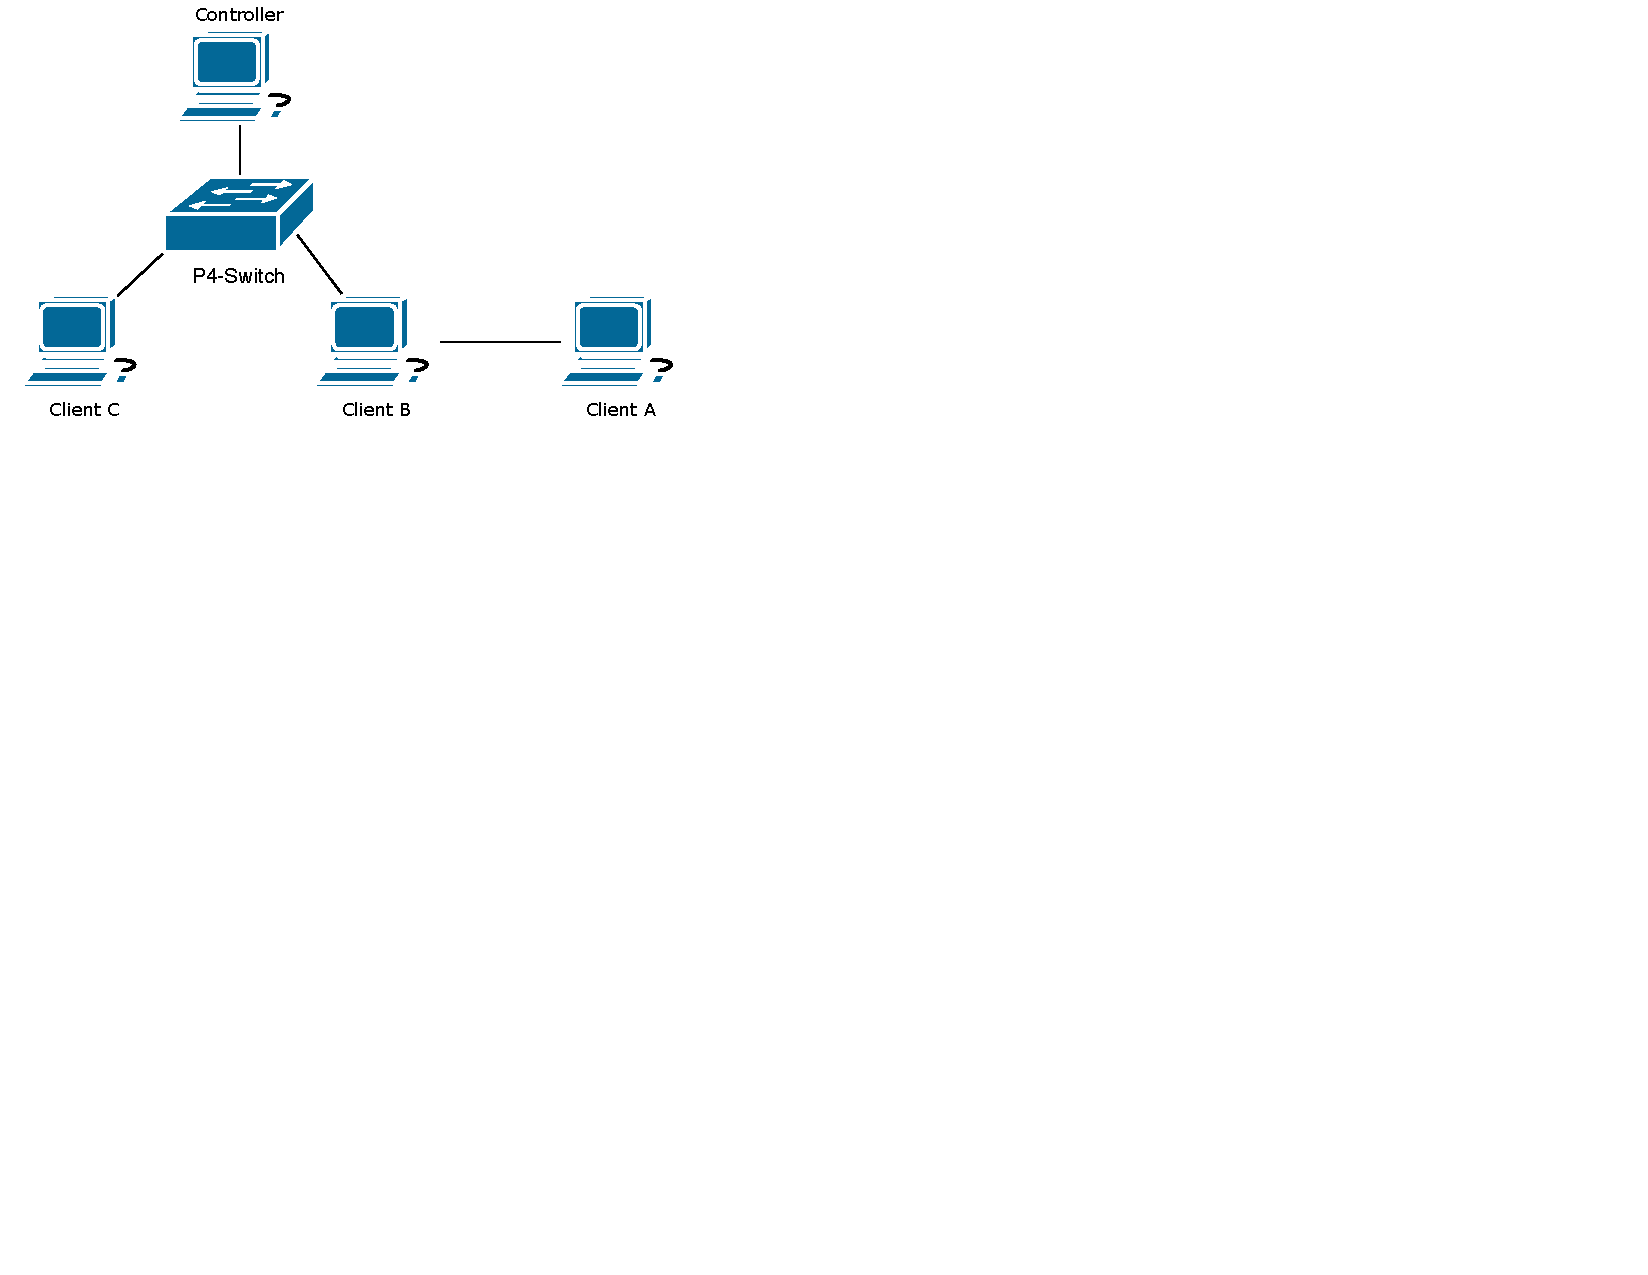
\includegraphics[width=0.5\textwidth]{Figures/Test_setup.pdf}
	  \end{center}

  \caption[Overview of the test setup used for the evaluation.]{Overview of the test setup used for the evaluation. Client A is a \textit{regular bitcoin client} that has 1 block that clients B/C and the\textit{controller} do not posses. Clients B and C are \textit{modified bitcoin clients}. The switch is a programmable P4-switch emulated in software.}
  \label{figure:test_setup}
\end{figure}

\section{\label{evaluation:setup}Functional evaluation}
Using mininet, a small test setup was created. The setup consists of 3 clients, one switch and a controller. An overview of the setup can be seen in figure \ref{figure:test_setup}. Client A is a \textit{regular bitcoin client} and clients B and C are \textit{modified bitcoin clients}. The controller is a bitcoin relay \textit{controller} as described in section \ref{design:SwitchController}. The test covers 2 important use cases. First, it shows that the \textit{modified client} is able to interact with the \textit{regular bitcoin client} and that therefore an incremental deployment in the bitcoin network is possible. Second, the update and advertisement process described in the \textit{relay protocol} is tested. 
\subsubsection{Setup}
The experiment goes through the following steps.
\begin{enumerate}
	\item Client A has a block that the other clients and the controller do not yet have in their local storage.
	\item Clients B and C do a handshake with the switch.
	\item Client A establishes a connection to client B.
	\item Client A advertises its latest block to client B using the regular bitcoin network protocol.
	\item Upon receiving the block, client B advertises the block to the switch.
	\item The switch does not know the block and sends a CTR message to client B indicating that it should connect to the controller.
	\item Client B establishes a connection to the controller.
	\item Client B sends its latest block to the controller using the regular bitcoin network protocol.
	\item The controller updates the switch and advertises the new block to all clients.
	\item Client C does not have the block in its local storage and requests the block from the switch and adds it to its chain.
\end{enumerate}
Note that there is no direct connection between clients B and C. To make sure that clients A and B establish a connection, the IP of client A was whitelisted at client B.\\
This setting was run with 10 different blocks and was repeated 20 times for each block which results in a total of 200 experiment runs. The mean block size was 1128194 bytes during the experiment. This means that there are 2261 segments in average.\\
\subsubsection{Results}
After each run, the log files that are generated by the clients and the controller are analysed. From this data, we can calculate the time needed for the block to travel from node B through the controller and the switch to client C.\\
We are interested in the time client B needs to connect to the controller. For this, we measure the time between the moment when client B adds a new block to the chain until the moment when the connection between the client and the controller is established. We see that after 2ms, the client sends an ADV message and receives a CON response from the switch 2ms later. The client then needs 11ms to connect to the controller. So in total, the client is connected 15ms after it received the block. After connecting, the client and the controller need 4.7s to transfer the new block from the client to the controller.\\
At the controller, we want to measure the time needed to update the switch. For this we measure the time starting from the moment when the controller adds the new block to its chain until the last BLK message is sent. We focus on the work done at the controller and neglect the time of flight of the packet and the overhead at the switch. We measure an update time of 3.4s. Remember that a 1ms delay was introduced when sending the block segments. With 2261 segments this means that there is a 2.26s delay which explains a part of the overhead. 7ms after the last segment is sent, the RINV message to the client is sent.\\
Lastly, we want to see how fast client C can request the block from the switch. For this, we measure the time between the moment when client C receives the RINV message and the moment when the block is added to the chain. We see, that the last segment of the block arrives after 4.3s. Again, the 2.26 seconds of transmission delay has to be taken into account here. After that, 3.9s is needed to verify the block and add it to the chain. The overhead here stems from the fact that the client has to verify all transactions that are contained in the block because they were not previously available to the client. In total, the block request takes 8.3s from the moment the RINV message is received. This is 52\% slower than the transmission of the block from client B to the controller that was using the regular bitcoin protocol. 
The whole process, starting from the moment client B receives the block until client C receives it takes 16.3s. To speed up this process, one could first investigate, if the 1ms delay is needed in actual hardware. This would reduce the measured time by 4.5s. Further, a future adaption could allow storing of transactions at the switch which would reduce the time needed by client C to add the new block to its chain. However, most of the time overhead can be regarded as setup cost for the cache at the switch. A more realistic scenario would be, when there is not a single client C but many clients that are interested in the block and are able to request it in parallel.

% this is new
%t1=0.002152884665367122
%t2=0.004278595191682911
%t3=0.014793193372319689
%t4=4.667016932781028
%t5=8.025114057147498
%t6=8.032396441975308
%t7=8.033542145451593
%t8=12.373263397368422
%t9=16.311130394704353
%size=1128193.6666666667


\section{Scaling \label{evaluation:scaling}}
To inspect the scaling behaviour of the controller, a python based pseudo client is crated which will open 1'000 connections to the relay. The test setup is the same as in section \ref{evaluation:setup}, but with client C replaced by 1'000 clients. After the pseudo client has set up the connections, it waits for incoming RINV messages and logs the arrival time of the last incoming RINV message. We run the test with 3 different blocks and 3 runs each. The time needed to send the 1'000 RINV messages is 1.24s. There is a 1ms delay between each message which accounts for 1s of the time needed. If the delay can be removed when working with real hardware, the 1'000 RINV messages are expected to be sent out in 240ms. As we expect the switch to be able to process requests at line rate, we do not expect a large overhead for the clients to request the blocks from the switch. However, this claim could not be verified with the software emulated switch.\\
Next, the connection count is further increased and the system stats are measured. We use the same setup as in sections \ref{sec:perf_degen} and \ref{sec:generalResources} but use the relay controller. The measurement is made on \textit{device 1}. We let the setup connect to 30 regular nodes  and use a python client to add 10'000 relay connections by sending emulated CON messages. The rest of the test setup is equal to the one defined in the before mentioned sections. CPU, I/O, Swap and Memory measurements show no significant overhead over the setup without the 10'000 relay connections. The results of the measurement can be seen in table \ref{tab:evaluation:generalresources}. The measurement of the RTT shows 19'335$\mu s$, which is comparable to about 200-300 regular connections according to table \ref{tab:performance_degeneration}. The measured delay can be explained by the overhead that is generated, when a new block arrives. If we assume a block that is split into 2500 segments, there are 12'500 messages (INV and BLK) that are sent per block. As there is an artificial delay of 1ms after every message, this means that there is a 12.5s overhead for each block. We assume to be able to greatly reduce the overhead when using a hardware switch.







\begin{table}[tbp]
\begin{center}	
\begin{tabular}{l|l|l|r }
\textbf{category} & \textbf{Parameter} & \textbf{Unit} & \textbf{30} \\
\hline
CPU & User & \%             & 1.36 \\
    & Sys  & \%             & 0.79  \\
    & Idle & \%             & 97.43 \\
    & Context switches & /5s  & 1'454.08 \\
\hline
I/O & Interrupts & /5s       & 673.37 \\
    & Disk reads   & /5s     & 150.35 \\
    & Disk writes   & /5s    & 26.87 \\
    & I/O wait     & s/5s       & 0.48 \\
\hline
Swap & Swap   & KB          & 7.21 \\
\hline
Memory & Free memory  & KB          & 114'138 \\
       & used Buffer space  & KB    & 67'954.4 \\
\end{tabular}
\caption[General resource measurements of the modified bitcoin client.]{General resource usage measurement on \textit{device 1} when connected to 10'000 nodes via the relay.}
\label{tab:evaluation:generalresources}
\end{center}
\end{table}











\section{Bandwidth overhead\label{evaluation:messages}}
The current bitcoin protocol specifies different ways to transmit blocks from one client to another. Most of the optimisations aim at smaller block messages to be able to speed up the block distribution. The optimisations relay on prefetching transactions so that the client is able to pre-verify the transactions. This makes it difficult to compare the message of the relay transmitted block size to the one needed by the current bitcoin protocol. Instead, we calculate the overhead compared to a traditional block message.
\subsubsection{Client}
First, we focus on the overhead introduced by the protocol. The relay message protocol specifies a payload size of 499 bytes. If we define $s_i$ as the size of the block message (block + header) and $s_r$ as the total cumulated message size of all segments, we can express $s_r$ by adding the overhead of the new header per segment and the padding overhead to $s_i$
\begin{equation}
	s_r = s_i+ \left\lceil \frac{s_i}{499B} \right\rceil \cdot 5B + s_i \mbox{ mod } 499
\end{equation}
Currently, blocks have the size of about 1MB. If we assume $504B \ll s_i$, we can express the protocol overhead as  
\begin{equation} \label{eq:overhead}
	\frac{s_r}{s_i} \approx 1+\frac{5}{499} = 1.01
\end{equation}
The 499 maximum payload size is smaller than the most commonly used MTU of TCP. This means, that the transport layer also adds an overhead to the transmitted block size. We assume a commonly used MTU of 1500 bytes for the calculations. Further we assume 24 bytes Ethernet headers, 20 bytes IP headers, 20 bytes TCP headers and 8 bytes UDP headers. We denote the transmitted message size of the regular and the relay blocks as $t_i$ and $t_r$ respectively. We get the following expressions
\begin{equation}
	t_i = s_i + \left\lceil \frac{s_i}{1500} \right\rceil(24 + 20 + 20)B
\end{equation} 
\begin{equation}
	t_r = s_r + \left\lceil \frac{s_r}{499} \right\rceil(24 + 20 + 8)B
\end{equation} 
Assuming $1500B \ll s_i$ and $499B \ll s_r$, we can estimate the bandwidth overhead as
\begin{equation} \label{eq:throughput}
	\frac{t_r}{t_i}\approx \frac{s_r}{s_i} \cdot\frac{1+\frac{52}{499}}{1+\frac{64}{1500}} = 1.07
\end{equation}
This rough estimate shows that we can expect overhead of about 7\% when comparing to a minimal TCP based transmission. The overhead could be reduced if the protocol would be changed to support larger payloads than 499 bytes. However, as the discovery of a new block is a sporadic event, this should not pose a large drawback.\\
So far, only the bandwidth overhead of incoming messages were observed. As each segment of the block has to be requested, the protocol also generates overhead on the outgoing messages. We compare the total amount of outgoing messages to a single getdata message of the regular bitcoin protocol. Getdata was chosen over other block exchange mechanisms such as headers messages, because getdata has the smallest foodprint. This will give us an estimate on the upper bound on the overhead. The getdata message with a single block hash has a size of 61 bytes. Per 499 bytes of block, the modified client has to send a request of size 37 bytes. On the other hand, the regular client sends TCP ACKs. If we assume a block of size 1MB, a TCP MTU of 1500B, 24B ethernet headers, 20B IP headers and 8B UDP headers and assume a lossless transmission, we get the following overhead:
\begin{equation}
	\frac{\left\lceil \frac{1MB}{499B} \right\rceil \cdot (37B + 52B)}{61B + 64B + \left\lceil \frac{1MB}{1500B} \right\rceil\cdot 64B} = 4.2
\end{equation}
In other words, the request size is increased by the factor 4.2 when comparing the relay protocol to the regular bitcoin protocol. This is limited by the protocol and can only be changed when changing the protocol or when increasing the data chunk size of the segments. However, as the requests of the individual segments is pipelined, this does not lead to a large overhead time wise. 



\subsubsection{Controller}
To send blocks, the controller has to update the switch. Similarly to equations \ref{eq:overhead} and \ref{eq:throughput}, the overhead can be calculated. Here, we have to add the overhead from the UPD message (35 bytes) and the additional checksum in the headers of the BLK messages (+2 bytes). However, as we have $35B \ll s_i$ and $\frac{5}{499}\approx\frac{7}{499}$, we get
\begin{equation}
	\frac{s_r}{s_i} \approx 1+\frac{7}{499} = 1.014
\end{equation}
and 
\begin{equation} \label{eq:throughput}
	\frac{t_r}{t_i}\approx \frac{s_r}{s_i} \cdot\frac{1+\frac{52}{499}}{1+\frac{64}{1500}} = 1.074
\end{equation}
for the outgoing message overhead.\\
The update process has to be done once per block. Except from the single 37 byte INV message per client, there is no additional overhead when the block is sent to multiple clients. This is a clear benefit when compared to the regular client, which needs to send the block for each peer that requests it.





















\section{Memory overhead \label{evaluation:memory}}
Let's first inspect the memory usage of the controller.
Let $m_0$ be the amount of memory needed to store the state of a single peer-to-peer connection. Let $m_b^n$ and $m_r^n$ be the amount of memory needed to store the state of n peer-to-peer connections and n relay connections, respectively. To maintain the basic connection to the relay, we use the same data structure as used by peer-to-peer connections. The connection uses a UDP connection instead of a TCP connection which uses less state, therefore we can say that
\begin{equation}
	m_r^0 \leq m_b^1 = m_0
\end{equation}
When adding new connections, a new data structure is added for the regular connections. For the relay connections, the metadata of the the peer is stored in the existing data structure. This leads to the following overhead
\begin{equation}
	m_b^n = n\cdot m_0
\end{equation}
\begin{equation}
	m_r^n = m_0 + n\cdot 6B
\end{equation}
While the actual size of the data structure can vary across compilers and operating systems, with gcc 5.4.0 on Ubuntu 16.04.1 we have $m_0 = 1672B$. This means that we use less than 1\% of the size of regular connections for the relay connections.\\
On the client, the connection to the switch uses the same data structure as regular connections. This means, that the memory usage is the same in user space. In kernel space, the memory overhead is smaller, because the UDP connection that is used needs to store less state.







\section{CPU overhead\label{evaluation:cpu}}
To measure the CPU overhead of the design, we use the same test setup as in section \ref{sec:workAnalysis}. We let the node establish 30 connections and add 10'000 relay connections using a pseudo client which emulates the CON messages from the switch before starting the profiler. Again, we let the experiment run for 4h and repeat it 3 times. The addition to the system accounts for 3.1\% of the total CPU time of the MessageHandler thread. From the results we can see that there is no significant overhead in adding 10'000 relay connections.





\section{Conclusion}
With this evaluation, we show that the presented solution has better scalability characteristics than the state-of-the-art bitcoin client. It was shown that the controller can handle multiple thousands of connections with a minimal memory and CPU overhead. The tradeoff for this increased scalability is the increased bandwidth needed by the clients and the slower block propagation. We expect to greatly improve the block propagation speed when running with a hardware switch instead of an emulated one.






















%** Outlook.tex: What needs to be done further, what is planed
%
\chapter{\label{outlook}Future Work}
The proposed modifications to the bitcoin client and the design of the controller can be used in the SABRE framework to protect against routing based network isolation attacks. The next step would be to perform a real world experiment using physical hardware for the switch. If this experiment shows promising results, the presented prototype can be used as a starting point for a real world implementation by addressing the design shortcomings mentioned in section \ref{sec:design:shortcomings}.\\
It would be interesting to see if modifications used by FIBRE can be used to improve the SABRE framework in terms of update and distribution speed. Additionally, the update delay of the SABRE framework could be improved by adding support for transactions and compact blocks in a future iteration.\\


%** Summary.tex: What have you achieved, what have you presented in this
%                document.  What are the highlights of your work.
%                It should conclude by a conclusion.
\chapter{\label{summary}Summary}
In this thesis we proposed a modified bitcoin client for the use with the SABRE framework. In chapter \ref{profiling}, we have shown that the current state-of-the-art has bad scaling properties. Using various measurements we were able to gradually pinpoint the bottleneck in scaling up to be the inter-thread communication. We defined properties that a modified bitcoin client should have. We presented a design for a modified bitcoin client that has these properties in in chapter \ref{design}. Additionally, a controller for the switch used in the SABRE network was designed. The shortcomings of the current design and security concerns were briefly discussed in section \ref{sec:design:shortcomings}. Using our prototype, we were able to show the improved scaling properties in chapter \ref{evaluation} by testing our implementation with up to 10'000 connections. We also showed, that the controller has desirable scaling properties in terms of memory usage and CPU overhead and showed the tradeoff between the scalability and the block distribution speed. We concluded this thesis with a short discussion about possible research directions in chapter \ref{outlook}.



%** Switch to appendix-mode in Latex.
%
\appendix

%** I would like to have the appendices enumerated by Alphabetical
%   characters.
\renewcommand{\thepart}{\Alph{part}}

%** appendix.tex: Install instructions, configurations, test results,
%		simulation data, additional theoretical disquisitions, ...
%
%%****************************************************************************
%** Copyright 2005 by Bernhard Tellenbach, <bernhard.tellenbach@airmail.ch>
%** Information is provided under the terms of the
%** GNU Free Documentation License <http://www.gnu.org/copyleft/fdl.html>
%****************************************************************************
%****************************************************************************
%** Last Modification: 2005-07-11 1600
%** 2005-07-11	Updated the syntax to match the current nomencl packet
%****************************************************************************

\chapter{\label{appendixMessagingProtocol}Relay Messaging Protocol}
The following table shows the exact specification of the different message types used in the \textit{relay protocol}. The field sizes and the communication directions are given in the corresponding columns.

\begin{center}
\begin{tabular}{|l|l|l|l|}
	\hline
	\textbf{Message Type} & \textbf{Communication} & \textbf{Size (bits)} & \textbf{Field} \\
	\hline
	REY	& C $\leftrightarrow$ S 	& 24		& Command (=REY) \\
		& 		& 4		& Flag \\
		& 		& 20		& Secret \\
	\hline
	INV	& M $\to$ C 	& 24		& Command (=INV) \\
		& 		& 256	& Block hash \\
		& 		& 16	& Segment count \\
		\hline
	SEG	& C $\to$ S 	& 24	& Command (=SEG) \\
		& 				& 256	& Block hash \\
		& 				& 16	& Segment id \\
		\hline
	BLK	& S $\to$ C 	& 24	& Command (=BLK)\\
		& 				& 16	& Segment id \\
		& 				& 499*8	& Segment data \\
		\hline
	BLK	& M $\to$ S 	& 24	& Command (=BLK)\\
		& 				& 16	& Segment id \\
		& 				& 499*8	& Segment data \\
		&				& 16	& precomputed UDP checksum \\
\hline
	ADV	& C $\to$ S 	& 24	& Command (=ADV)\\
		& 				& 256	& Block hash \\
\hline
	CTR	& S $\to$ C 	& 24	& Command (=CTR)\\
		& 				& 32	& IP \\
		& 				& 16	& port \\
		&				& 8		& empty \\
\hline
	CON	& S $\to$ M 	& 24	& Command (=CON) \\
		& 				& 8		& empty \\
		& 				& 16	& port \\
		& 				& 32	& IP \\
\hline
	UPD	& M $\to$ S 	& 24	& Command (=UPD) \\
		& 				& 256	& Block hash \\
\hline
	BCL	& M $\to$ S 	& 24	& Command (=BCL) \\
		& 				& 32	& ip \\
	\hline
\end{tabular}\\
\end{center}
M: Controller\\
S: Switch\\
C: Client\\




\chapter{\label{appendix:pingClient}Ping Client Modifications}
The following code alterations are made to create the \textit{ping client} from the regular bitcoin client. 


\begin{diffCode}
diff --git a/src/net.h b/src/net.h
index 8378a303b..cd1dda236 100644
--- a/src/net.h
+++ b/src/net.h
@@ -38,7 +38,7 @@ class CScheduler;
 class CNode;

 /** Time between pings automatically sent out for latency probing and keepalive (in seconds). */
-static const int PING_INTERVAL = 2 * 60;
+static const int PING_INTERVAL = 1;
 /** Time after which to disconnect, after waiting for a ping response (or inactivity). */
 static const int TIMEOUT_INTERVAL = 20 * 60;
 /** Run the feeler connection loop once every 2 minutes or 120 seconds. **/
diff --git a/src/net_processing.cpp b/src/net_processing.cpp
index bf9307727..de2ced1ae 100644
--- a/src/net_processing.cpp
+++ b/src/net_processing.cpp
@@ -2720,6 +2720,7 @@ bool static ProcessMessage(CNode* pfrom, const std::string& strCommand, CDataStr

     else if (strCommand == NetMsgType::PONG)
     {
+	LogPrintf("THROUGHPUT: PONG: %u\n", GetTimeMicros());
         int64_t pingUsecEnd = nTimeReceived;
         uint64_t nonce = 0;
         size_t nAvail = vRecv.in_avail();
@@ -3175,6 +3176,7 @@ bool PeerLogicValidation::SendMessages(CNode* pto, std::atomic<bool>& interruptM
         }
         if (pto->nPingNonceSent == 0 && pto->nPingUsecStart + PING_INTERVAL * 1000000 < GetTimeMicros()) {
             // Ping automatically sent as a latency probe & keepalive.
+	    LogPrintf("THROUGHPUT: PING: %u\n", GetTimeMicros());
             pingSend = true;
         }
         if (pingSend) {
@@ -3194,6 +3196,8 @@ bool PeerLogicValidation::SendMessages(CNode* pto, std::atomic<bool>& interruptM
             }
         }

+	return true;
+
         TRY_LOCK(cs_main, lockMain); // Acquire cs_main for IsInitialBlockDownload() and CNodeState()
         if (!lockMain)
             return true;	
\end{diffCode}












%Entries for the list of abbrevations:
%
%To generate the list of abbrevations, execute:
%makeindex Thesis.nlo -s nomencl.ist -o Thesis.nls
%
%If you are using TeXniCenter, specify:
%"%bm.nlo" -s nomencl.ist -o "%bm.nls"
%as beeing the argument list for makeindex.
%---------------------------------------------------------------------------------------------------------
%For old nomencl package uncomment this:
%\printglossary
%For new nomencl package uncomment this:
\printnomenclature

\abbrev{XCA}{\markup{X}tremely \markup{C}ool \markup{A}bbrevations}





%** bibtex is used to automatically generate the bibliography
%   references are stored in refs/refs.bib
%   use a bibliography manager like JabRef (http://jabref.sourceforge.net/) to manage refs/refs.bib
\bibliographystyle{ieeetr}
\bibliography{refs/refs}

%** end the document environment
\end{document}
